% Seminar 3: Distribuții Stabile
% Statistica Piețelor Financiare

\documentclass[9pt, aspectratio=169, t]{beamer}
%=============================================================================
% PREAMBUL COMUN - Statistica Piețelor Financiare
% Prezentări academice de calitate Harvard
% Program de licență, Academia de Studii Economice din București
%
% Utilizare: \documentclass[9pt, aspectratio=169, t]{beamer}
%            %=============================================================================
% PREAMBUL COMUN - Statistica Piețelor Financiare
% Prezentări academice de calitate Harvard
% Program de licență, Academia de Studii Economice din București
%
% Utilizare: \documentclass[9pt, aspectratio=169, t]{beamer}
%            %=============================================================================
% PREAMBUL COMUN - Statistica Piețelor Financiare
% Prezentări academice de calitate Harvard
% Program de licență, Academia de Studii Economice din București
%
% Utilizare: \documentclass[9pt, aspectratio=169, t]{beamer}
%            \input{preamble}
%            \subtitle{Seminar X: Titlul Seminarului}
%            \begin{document} ...
%=============================================================================

% Asigură încadrarea conținutului pe diapozitive
\setbeamersize{text margin left=8mm, text margin right=8mm}

%=============================================================================
% CONFIGURARE TEMĂ ȘI STIL
%=============================================================================
\usetheme{default}

% Paletă de Culori
\definecolor{MainBlue}{RGB}{26, 58, 110}
\definecolor{AccentBlue}{RGB}{26, 58, 110}
\definecolor{IDAred}{RGB}{205, 0, 0}
\definecolor{DarkGray}{RGB}{51, 51, 51}
\definecolor{MediumGray}{RGB}{128, 128, 128}
\definecolor{LightGray}{RGB}{248, 248, 248}
\definecolor{VeryLightGray}{RGB}{235, 235, 235}
\definecolor{KeynoteGray}{RGB}{218, 218, 218}
\definecolor{SectionGray}{RGB}{120, 120, 120}
\definecolor{FooterGray}{RGB}{100, 100, 100}
\definecolor{Crimson}{RGB}{220, 53, 69}
\definecolor{Forest}{RGB}{46, 125, 50}
\definecolor{Amber}{RGB}{181, 133, 63}
\definecolor{Orange}{RGB}{230, 126, 34}
\definecolor{Purple}{RGB}{142, 68, 173}

% Fundal gradient (gradient Keynote exact 315°: alb la RGB 218,218,218)
\setbeamertemplate{background}{%
    \begin{tikzpicture}[remember picture, overlay]
        \shade[shading=axis, shading angle=315,
        top color=white, bottom color=KeynoteGray]
        (current page.south west) rectangle (current page.north east);
    \end{tikzpicture}%
}
% Culoare solidă de rezervă pentru compatibilitate
\setbeamercolor{background canvas}{bg=}

\setbeamercolor{palette primary}{bg=MainBlue, fg=white}
\setbeamercolor{palette secondary}{bg=MainBlue!85, fg=white}
\setbeamercolor{palette tertiary}{bg=MainBlue!70, fg=white}
\setbeamercolor{structure}{fg=MainBlue}
\setbeamercolor{title}{fg=IDAred}
\setbeamercolor{frametitle}{fg=IDAred, bg=}
\setbeamercolor{block title}{bg=MainBlue, fg=white}
\setbeamercolor{block body}{bg=VeryLightGray, fg=DarkGray}
\setbeamercolor{block title alerted}{bg=Crimson, fg=white}
\setbeamercolor{block body alerted}{bg=Crimson!8, fg=DarkGray}
\setbeamercolor{block title example}{bg=Forest, fg=white}
\setbeamercolor{block body example}{bg=Forest!8, fg=DarkGray}
\setbeamercolor{item}{fg=MainBlue}

% Font institute mai mic pentru a evita overfull hbox pe pagina de titlu
\setbeamerfont{institute}{size=\footnotesize}

% Culori subsol
\setbeamercolor{author in head/foot}{fg=FooterGray, bg=}
\setbeamercolor{title in head/foot}{fg=FooterGray, bg=}
\setbeamercolor{date in head/foot}{fg=FooterGray, bg=}
\setbeamercolor{section in head/foot}{fg=FooterGray, bg=}
\setbeamercolor{subsection in head/foot}{fg=FooterGray, bg=}

% Stiluri marcatori
\setbeamertemplate{itemize item}{\color{MainBlue}$\boxdot$}
\setbeamertemplate{itemize subitem}{\color{MainBlue}$\blacktriangleright$}
\setbeamertemplate{itemize subsubitem}{\color{MainBlue}\tiny$\bullet$}
\setbeamertemplate{itemize/enumerate body begin}{\normalsize}
\setbeamertemplate{itemize/enumerate subbody begin}{\normalsize}

% Stiluri cuprins (bullets în loc de numere)
\setbeamertemplate{section in toc}{%
    \leavevmode\leftskip=1.5em%
    \llap{\color{MainBlue}$\boxdot$\kern0.5em}%
    \inserttocsection\par%
}

% Spațiere compactă
\setlength{\leftmargini}{10pt}
\setlength{\leftmarginii}{10pt}
\makeatletter
\def\@listi{\leftmargin\leftmargini \topsep 0pt \parsep 0pt \itemsep 0pt}
\def\@listii{\leftmargin\leftmarginii \topsep 0pt \parsep 0pt \itemsep 0pt}
\makeatother

\setbeamertemplate{navigation symbols}{}

%=============================================================================
% ANTET PERSONALIZAT
%=============================================================================
\setbeamertemplate{headline}{%
    \vskip10pt%
    \hbox to \paperwidth{%
        \hskip0.5cm%
        {\small\color{FooterGray}\renewcommand{\hyperlink}[2]{##2}\insertsectionhead}%
        \hfill%
        \textcolor{FooterGray}{\small\insertframenumber}%
        \hskip0.5cm%
    }%
    \vskip4pt%
    {\color{FooterGray}\hrule height 0.4pt}%
}

%=============================================================================
% SUBSOL PERSONALIZAT
%=============================================================================
\usepackage{fontawesome5}

\setbeamertemplate{footline}{%
    {\color{FooterGray}\hrule height 0.4pt}%
    \vskip4pt%
    \hbox to \paperwidth{%
        \hskip0.5cm%
        \textcolor{FooterGray}{\small Statistica Piețelor Financiare}%
        \hfill%
        \raisebox{-0.1em}{%
            \begin{tikzpicture}[x=0.08em, y=0.08em, line width=0.4pt]
                \draw[FooterGray] (0,3) -- (1,4) -- (2,3.5) -- (3,5) -- (4,4) -- (5,6) -- (6,5.5) -- (7,4) -- (8,5) -- (9,7) -- (10,6) -- (11,5) -- (12,6.5) -- (13,8) -- (14,7) -- (15,6) -- (16,7.5) -- (17,9) -- (18,8) -- (19,7) -- (20,8.5) -- (21,10) -- (22,9) -- (23,8) -- (24,9.5);
            \end{tikzpicture}%
        }%
        \hskip0.5cm%
    }%
    \vskip6pt%
}

%=============================================================================
% PACHETE
%=============================================================================
\usepackage[utf8]{inputenc}
\usepackage[T1]{fontenc}
\usepackage{amsmath, amssymb, amsthm}
\usepackage{mathtools}
\usepackage{bm}
\usepackage{tikz}
\usetikzlibrary{arrows.meta, positioning, shapes, calc, decorations.pathreplacing, shadings}
\usepackage{booktabs}
\usepackage{multirow}
\usepackage{array}
\usepackage{graphicx}
\usepackage{hyperref}
\usepackage{colortbl}
\usepackage{listings}
\lstset{basicstyle=\ttfamily\small, breaklines=true, frame=single, backgroundcolor=\color{VeryLightGray}}
\hypersetup{colorlinks=true, linkcolor=MainBlue, urlcolor=MainBlue}
\graphicspath{{../../logos/}{../../charts/}{../../photos/}}
\hfuzz=2pt
\vfuzz=2pt

%=============================================================================
% COMANDA QUANTLET
%=============================================================================
\newcommand{\quantlet}[2]{%
    \hfill\href{#2}{%
        \raisebox{-0.15em}{
\includegraphics[height=0.7em]{ql_logo.png}}%
        \textcolor{MainBlue}{\tiny\ #1}%
    }%
}

%=============================================================================
% PAGINĂ TITLU PERSONALIZATĂ
%=============================================================================
\defbeamertemplate*{title page}{hybrid}[1][]
{
    \vspace{0.2cm}
    \begin{center}
        \href{https://www.ase.ro}{
\includegraphics[height=1.0cm]{ase_logo.png}}\hspace{0.25cm}%
        \href{https://theida.net}{
\includegraphics[height=1.0cm]{ida_logo.png}}\hspace{0.25cm}%
        \href{https://blockchain-research-center.com}{
\includegraphics[height=1.0cm]{brc_logo.png}}\hspace{0.25cm}%
        \href{https://www.ai4efin.ase.ro}{
\includegraphics[height=1.0cm]{ai4efin_logo.png}}\hspace{0.25cm}%
        \href{https://ipe.ro/new}{
\includegraphics[height=1.0cm]{acad_logo.png}}\hspace{0.25cm}%
        \href{https://www.digital-finance-msca.com}{
\includegraphics[height=1.0cm]{msca_logo.png}}%
    \end{center}

    \vspace{0.6cm}

    \begin{center}
        \begin{minipage}{0.1\textwidth}
            \centering
            \href{https://quantlet.com}{
\includegraphics[height=1.1cm]{ql_logo.png}}
        \end{minipage}%
        \begin{minipage}{0.78\textwidth}
            \centering
            {\LARGE\bfseries\usebeamercolor[fg]{title}\inserttitle}

            \vspace{0.3cm}

            {\usebeamerfont{subtitle}\usebeamercolor[fg]{title}\insertsubtitle}
        \end{minipage}%
        \begin{minipage}{0.1\textwidth}
            \centering
            \href{https://quantinar.com}{
\includegraphics[height=1.1cm]{qr_logo.png}}
        \end{minipage}
    \end{center}

    \vspace{0.6cm}

    \hspace{0.5cm}{\usebeamerfont{author}\insertauthor}

    \vspace{0.3cm}

    \hspace{0.5cm}\begin{minipage}[t]{0.9\textwidth}
        \raggedright\small\insertinstitute
    \end{minipage}
}

%=============================================================================
% MEDII PENTRU TEOREME
%=============================================================================
\theoremstyle{definition}
\setbeamertemplate{theorems}[numbered]
\newtheorem{defn}{Definiție}
\newtheorem{thm}{Teoremă}
\newtheorem{prop}{Propoziție}
\newtheorem{rmk}{Observație}

%=============================================================================
% CENTRED MINIPAGE
%=============================================================================
\newenvironment{cminipage}[1]{%
    \par\noindent\hfill\begin{minipage}{#1}\ignorespaces
}{%
    \end{minipage}\hfill\null\par
}

%=============================================================================
% COMENZI PERSONALIZATE
%=============================================================================
\newcommand{\E}{\mathbb{E}}
\newcommand{\Var}{\text{Var}}
\newcommand{\Cov}{\text{Cov}}
\newcommand{\Corr}{\text{Corr}}
\newcommand{\R}{\mathbb{R}}
\newcommand{\N}{\mathbb{N}}
\newcommand{\Z}{\mathbb{Z}}
\newcommand{\B}{\mathbf{B}}
\newcommand{\imark}{\textcolor{MainBlue}{\textbullet}}
\newcommand{\RMSE}{\text{RMSE}}
\newcommand{\MAE}{\text{MAE}}
\newcommand{\MAPE}{\text{MAPE}}
\newcommand{\correct}{\textcolor{Forest}{\checkmark}}
\newcommand{\incorrect}{\textcolor{Crimson}{\texttimes}}

%=============================================================================
% INFORMAȚII TITLU
%=============================================================================
\title[Statistica Piețelor Financiare]{Statistica Piețelor Financiare}
\author[D.T. Pele, A. Amza]{\texorpdfstring{\begin{tabular}[t]{@{}l@{}}Daniel Traian PELE \\ Antoaneta Amza\end{tabular}}{Daniel Traian PELE, Antoaneta Amza}}
\institute{Academia de Studii Economice din București\\
IDA Institute Digital Assets\\
Blockchain Research Center\\
AI4EFin Artificial Intelligence for Energy Finance\\
Academia Română, Institutul de Prognoză Economică\\
MSCA Digital Finance}
\date{}

%            \subtitle{Seminar X: Titlul Seminarului}
%            \begin{document} ...
%=============================================================================

% Asigură încadrarea conținutului pe diapozitive
\setbeamersize{text margin left=8mm, text margin right=8mm}

%=============================================================================
% CONFIGURARE TEMĂ ȘI STIL
%=============================================================================
\usetheme{default}

% Paletă de Culori
\definecolor{MainBlue}{RGB}{26, 58, 110}
\definecolor{AccentBlue}{RGB}{26, 58, 110}
\definecolor{IDAred}{RGB}{205, 0, 0}
\definecolor{DarkGray}{RGB}{51, 51, 51}
\definecolor{MediumGray}{RGB}{128, 128, 128}
\definecolor{LightGray}{RGB}{248, 248, 248}
\definecolor{VeryLightGray}{RGB}{235, 235, 235}
\definecolor{KeynoteGray}{RGB}{218, 218, 218}
\definecolor{SectionGray}{RGB}{120, 120, 120}
\definecolor{FooterGray}{RGB}{100, 100, 100}
\definecolor{Crimson}{RGB}{220, 53, 69}
\definecolor{Forest}{RGB}{46, 125, 50}
\definecolor{Amber}{RGB}{181, 133, 63}
\definecolor{Orange}{RGB}{230, 126, 34}
\definecolor{Purple}{RGB}{142, 68, 173}

% Fundal gradient (gradient Keynote exact 315°: alb la RGB 218,218,218)
\setbeamertemplate{background}{%
    \begin{tikzpicture}[remember picture, overlay]
        \shade[shading=axis, shading angle=315,
        top color=white, bottom color=KeynoteGray]
        (current page.south west) rectangle (current page.north east);
    \end{tikzpicture}%
}
% Culoare solidă de rezervă pentru compatibilitate
\setbeamercolor{background canvas}{bg=}

\setbeamercolor{palette primary}{bg=MainBlue, fg=white}
\setbeamercolor{palette secondary}{bg=MainBlue!85, fg=white}
\setbeamercolor{palette tertiary}{bg=MainBlue!70, fg=white}
\setbeamercolor{structure}{fg=MainBlue}
\setbeamercolor{title}{fg=IDAred}
\setbeamercolor{frametitle}{fg=IDAred, bg=}
\setbeamercolor{block title}{bg=MainBlue, fg=white}
\setbeamercolor{block body}{bg=VeryLightGray, fg=DarkGray}
\setbeamercolor{block title alerted}{bg=Crimson, fg=white}
\setbeamercolor{block body alerted}{bg=Crimson!8, fg=DarkGray}
\setbeamercolor{block title example}{bg=Forest, fg=white}
\setbeamercolor{block body example}{bg=Forest!8, fg=DarkGray}
\setbeamercolor{item}{fg=MainBlue}

% Font institute mai mic pentru a evita overfull hbox pe pagina de titlu
\setbeamerfont{institute}{size=\footnotesize}

% Culori subsol
\setbeamercolor{author in head/foot}{fg=FooterGray, bg=}
\setbeamercolor{title in head/foot}{fg=FooterGray, bg=}
\setbeamercolor{date in head/foot}{fg=FooterGray, bg=}
\setbeamercolor{section in head/foot}{fg=FooterGray, bg=}
\setbeamercolor{subsection in head/foot}{fg=FooterGray, bg=}

% Stiluri marcatori
\setbeamertemplate{itemize item}{\color{MainBlue}$\boxdot$}
\setbeamertemplate{itemize subitem}{\color{MainBlue}$\blacktriangleright$}
\setbeamertemplate{itemize subsubitem}{\color{MainBlue}\tiny$\bullet$}
\setbeamertemplate{itemize/enumerate body begin}{\normalsize}
\setbeamertemplate{itemize/enumerate subbody begin}{\normalsize}

% Stiluri cuprins (bullets în loc de numere)
\setbeamertemplate{section in toc}{%
    \leavevmode\leftskip=1.5em%
    \llap{\color{MainBlue}$\boxdot$\kern0.5em}%
    \inserttocsection\par%
}

% Spațiere compactă
\setlength{\leftmargini}{10pt}
\setlength{\leftmarginii}{10pt}
\makeatletter
\def\@listi{\leftmargin\leftmargini \topsep 0pt \parsep 0pt \itemsep 0pt}
\def\@listii{\leftmargin\leftmarginii \topsep 0pt \parsep 0pt \itemsep 0pt}
\makeatother

\setbeamertemplate{navigation symbols}{}

%=============================================================================
% ANTET PERSONALIZAT
%=============================================================================
\setbeamertemplate{headline}{%
    \vskip10pt%
    \hbox to \paperwidth{%
        \hskip0.5cm%
        {\small\color{FooterGray}\renewcommand{\hyperlink}[2]{##2}\insertsectionhead}%
        \hfill%
        \textcolor{FooterGray}{\small\insertframenumber}%
        \hskip0.5cm%
    }%
    \vskip4pt%
    {\color{FooterGray}\hrule height 0.4pt}%
}

%=============================================================================
% SUBSOL PERSONALIZAT
%=============================================================================
\usepackage{fontawesome5}

\setbeamertemplate{footline}{%
    {\color{FooterGray}\hrule height 0.4pt}%
    \vskip4pt%
    \hbox to \paperwidth{%
        \hskip0.5cm%
        \textcolor{FooterGray}{\small Statistica Piețelor Financiare}%
        \hfill%
        \raisebox{-0.1em}{%
            \begin{tikzpicture}[x=0.08em, y=0.08em, line width=0.4pt]
                \draw[FooterGray] (0,3) -- (1,4) -- (2,3.5) -- (3,5) -- (4,4) -- (5,6) -- (6,5.5) -- (7,4) -- (8,5) -- (9,7) -- (10,6) -- (11,5) -- (12,6.5) -- (13,8) -- (14,7) -- (15,6) -- (16,7.5) -- (17,9) -- (18,8) -- (19,7) -- (20,8.5) -- (21,10) -- (22,9) -- (23,8) -- (24,9.5);
            \end{tikzpicture}%
        }%
        \hskip0.5cm%
    }%
    \vskip6pt%
}

%=============================================================================
% PACHETE
%=============================================================================
\usepackage[utf8]{inputenc}
\usepackage[T1]{fontenc}
\usepackage{amsmath, amssymb, amsthm}
\usepackage{mathtools}
\usepackage{bm}
\usepackage{tikz}
\usetikzlibrary{arrows.meta, positioning, shapes, calc, decorations.pathreplacing, shadings}
\usepackage{booktabs}
\usepackage{multirow}
\usepackage{array}
\usepackage{graphicx}
\usepackage{hyperref}
\usepackage{colortbl}
\usepackage{listings}
\lstset{basicstyle=\ttfamily\small, breaklines=true, frame=single, backgroundcolor=\color{VeryLightGray}}
\hypersetup{colorlinks=true, linkcolor=MainBlue, urlcolor=MainBlue}
\graphicspath{{../../logos/}{../../charts/}{../../photos/}}
\hfuzz=2pt
\vfuzz=2pt

%=============================================================================
% COMANDA QUANTLET
%=============================================================================
\newcommand{\quantlet}[2]{%
    \hfill\href{#2}{%
        \raisebox{-0.15em}{
\includegraphics[height=0.7em]{ql_logo.png}}%
        \textcolor{MainBlue}{\tiny\ #1}%
    }%
}

%=============================================================================
% PAGINĂ TITLU PERSONALIZATĂ
%=============================================================================
\defbeamertemplate*{title page}{hybrid}[1][]
{
    \vspace{0.2cm}
    \begin{center}
        \href{https://www.ase.ro}{
\includegraphics[height=1.0cm]{ase_logo.png}}\hspace{0.25cm}%
        \href{https://theida.net}{
\includegraphics[height=1.0cm]{ida_logo.png}}\hspace{0.25cm}%
        \href{https://blockchain-research-center.com}{
\includegraphics[height=1.0cm]{brc_logo.png}}\hspace{0.25cm}%
        \href{https://www.ai4efin.ase.ro}{
\includegraphics[height=1.0cm]{ai4efin_logo.png}}\hspace{0.25cm}%
        \href{https://ipe.ro/new}{
\includegraphics[height=1.0cm]{acad_logo.png}}\hspace{0.25cm}%
        \href{https://www.digital-finance-msca.com}{
\includegraphics[height=1.0cm]{msca_logo.png}}%
    \end{center}

    \vspace{0.6cm}

    \begin{center}
        \begin{minipage}{0.1\textwidth}
            \centering
            \href{https://quantlet.com}{
\includegraphics[height=1.1cm]{ql_logo.png}}
        \end{minipage}%
        \begin{minipage}{0.78\textwidth}
            \centering
            {\LARGE\bfseries\usebeamercolor[fg]{title}\inserttitle}

            \vspace{0.3cm}

            {\usebeamerfont{subtitle}\usebeamercolor[fg]{title}\insertsubtitle}
        \end{minipage}%
        \begin{minipage}{0.1\textwidth}
            \centering
            \href{https://quantinar.com}{
\includegraphics[height=1.1cm]{qr_logo.png}}
        \end{minipage}
    \end{center}

    \vspace{0.6cm}

    \hspace{0.5cm}{\usebeamerfont{author}\insertauthor}

    \vspace{0.3cm}

    \hspace{0.5cm}\begin{minipage}[t]{0.9\textwidth}
        \raggedright\small\insertinstitute
    \end{minipage}
}

%=============================================================================
% MEDII PENTRU TEOREME
%=============================================================================
\theoremstyle{definition}
\setbeamertemplate{theorems}[numbered]
\newtheorem{defn}{Definiție}
\newtheorem{thm}{Teoremă}
\newtheorem{prop}{Propoziție}
\newtheorem{rmk}{Observație}

%=============================================================================
% CENTRED MINIPAGE
%=============================================================================
\newenvironment{cminipage}[1]{%
    \par\noindent\hfill\begin{minipage}{#1}\ignorespaces
}{%
    \end{minipage}\hfill\null\par
}

%=============================================================================
% COMENZI PERSONALIZATE
%=============================================================================
\newcommand{\E}{\mathbb{E}}
\newcommand{\Var}{\text{Var}}
\newcommand{\Cov}{\text{Cov}}
\newcommand{\Corr}{\text{Corr}}
\newcommand{\R}{\mathbb{R}}
\newcommand{\N}{\mathbb{N}}
\newcommand{\Z}{\mathbb{Z}}
\newcommand{\B}{\mathbf{B}}
\newcommand{\imark}{\textcolor{MainBlue}{\textbullet}}
\newcommand{\RMSE}{\text{RMSE}}
\newcommand{\MAE}{\text{MAE}}
\newcommand{\MAPE}{\text{MAPE}}
\newcommand{\correct}{\textcolor{Forest}{\checkmark}}
\newcommand{\incorrect}{\textcolor{Crimson}{\texttimes}}

%=============================================================================
% INFORMAȚII TITLU
%=============================================================================
\title[Statistica Piețelor Financiare]{Statistica Piețelor Financiare}
\author[D.T. Pele, A. Amza]{\texorpdfstring{\begin{tabular}[t]{@{}l@{}}Daniel Traian PELE \\ Antoaneta Amza\end{tabular}}{Daniel Traian PELE, Antoaneta Amza}}
\institute{Academia de Studii Economice din București\\
IDA Institute Digital Assets\\
Blockchain Research Center\\
AI4EFin Artificial Intelligence for Energy Finance\\
Academia Română, Institutul de Prognoză Economică\\
MSCA Digital Finance}
\date{}

%            \subtitle{Seminar X: Titlul Seminarului}
%            \begin{document} ...
%=============================================================================

% Asigură încadrarea conținutului pe diapozitive
\setbeamersize{text margin left=8mm, text margin right=8mm}

%=============================================================================
% CONFIGURARE TEMĂ ȘI STIL
%=============================================================================
\usetheme{default}

% Paletă de Culori
\definecolor{MainBlue}{RGB}{26, 58, 110}
\definecolor{AccentBlue}{RGB}{26, 58, 110}
\definecolor{IDAred}{RGB}{205, 0, 0}
\definecolor{DarkGray}{RGB}{51, 51, 51}
\definecolor{MediumGray}{RGB}{128, 128, 128}
\definecolor{LightGray}{RGB}{248, 248, 248}
\definecolor{VeryLightGray}{RGB}{235, 235, 235}
\definecolor{KeynoteGray}{RGB}{218, 218, 218}
\definecolor{SectionGray}{RGB}{120, 120, 120}
\definecolor{FooterGray}{RGB}{100, 100, 100}
\definecolor{Crimson}{RGB}{220, 53, 69}
\definecolor{Forest}{RGB}{46, 125, 50}
\definecolor{Amber}{RGB}{181, 133, 63}
\definecolor{Orange}{RGB}{230, 126, 34}
\definecolor{Purple}{RGB}{142, 68, 173}

% Fundal gradient (gradient Keynote exact 315°: alb la RGB 218,218,218)
\setbeamertemplate{background}{%
    \begin{tikzpicture}[remember picture, overlay]
        \shade[shading=axis, shading angle=315,
        top color=white, bottom color=KeynoteGray]
        (current page.south west) rectangle (current page.north east);
    \end{tikzpicture}%
}
% Culoare solidă de rezervă pentru compatibilitate
\setbeamercolor{background canvas}{bg=}

\setbeamercolor{palette primary}{bg=MainBlue, fg=white}
\setbeamercolor{palette secondary}{bg=MainBlue!85, fg=white}
\setbeamercolor{palette tertiary}{bg=MainBlue!70, fg=white}
\setbeamercolor{structure}{fg=MainBlue}
\setbeamercolor{title}{fg=IDAred}
\setbeamercolor{frametitle}{fg=IDAred, bg=}
\setbeamercolor{block title}{bg=MainBlue, fg=white}
\setbeamercolor{block body}{bg=VeryLightGray, fg=DarkGray}
\setbeamercolor{block title alerted}{bg=Crimson, fg=white}
\setbeamercolor{block body alerted}{bg=Crimson!8, fg=DarkGray}
\setbeamercolor{block title example}{bg=Forest, fg=white}
\setbeamercolor{block body example}{bg=Forest!8, fg=DarkGray}
\setbeamercolor{item}{fg=MainBlue}

% Font institute mai mic pentru a evita overfull hbox pe pagina de titlu
\setbeamerfont{institute}{size=\footnotesize}

% Culori subsol
\setbeamercolor{author in head/foot}{fg=FooterGray, bg=}
\setbeamercolor{title in head/foot}{fg=FooterGray, bg=}
\setbeamercolor{date in head/foot}{fg=FooterGray, bg=}
\setbeamercolor{section in head/foot}{fg=FooterGray, bg=}
\setbeamercolor{subsection in head/foot}{fg=FooterGray, bg=}

% Stiluri marcatori
\setbeamertemplate{itemize item}{\color{MainBlue}$\boxdot$}
\setbeamertemplate{itemize subitem}{\color{MainBlue}$\blacktriangleright$}
\setbeamertemplate{itemize subsubitem}{\color{MainBlue}\tiny$\bullet$}
\setbeamertemplate{itemize/enumerate body begin}{\normalsize}
\setbeamertemplate{itemize/enumerate subbody begin}{\normalsize}

% Stiluri cuprins (bullets în loc de numere)
\setbeamertemplate{section in toc}{%
    \leavevmode\leftskip=1.5em%
    \llap{\color{MainBlue}$\boxdot$\kern0.5em}%
    \inserttocsection\par%
}

% Spațiere compactă
\setlength{\leftmargini}{10pt}
\setlength{\leftmarginii}{10pt}
\makeatletter
\def\@listi{\leftmargin\leftmargini \topsep 0pt \parsep 0pt \itemsep 0pt}
\def\@listii{\leftmargin\leftmarginii \topsep 0pt \parsep 0pt \itemsep 0pt}
\makeatother

\setbeamertemplate{navigation symbols}{}

%=============================================================================
% ANTET PERSONALIZAT
%=============================================================================
\setbeamertemplate{headline}{%
    \vskip10pt%
    \hbox to \paperwidth{%
        \hskip0.5cm%
        {\small\color{FooterGray}\renewcommand{\hyperlink}[2]{##2}\insertsectionhead}%
        \hfill%
        \textcolor{FooterGray}{\small\insertframenumber}%
        \hskip0.5cm%
    }%
    \vskip4pt%
    {\color{FooterGray}\hrule height 0.4pt}%
}

%=============================================================================
% SUBSOL PERSONALIZAT
%=============================================================================
\usepackage{fontawesome5}

\setbeamertemplate{footline}{%
    {\color{FooterGray}\hrule height 0.4pt}%
    \vskip4pt%
    \hbox to \paperwidth{%
        \hskip0.5cm%
        \textcolor{FooterGray}{\small Statistica Piețelor Financiare}%
        \hfill%
        \raisebox{-0.1em}{%
            \begin{tikzpicture}[x=0.08em, y=0.08em, line width=0.4pt]
                \draw[FooterGray] (0,3) -- (1,4) -- (2,3.5) -- (3,5) -- (4,4) -- (5,6) -- (6,5.5) -- (7,4) -- (8,5) -- (9,7) -- (10,6) -- (11,5) -- (12,6.5) -- (13,8) -- (14,7) -- (15,6) -- (16,7.5) -- (17,9) -- (18,8) -- (19,7) -- (20,8.5) -- (21,10) -- (22,9) -- (23,8) -- (24,9.5);
            \end{tikzpicture}%
        }%
        \hskip0.5cm%
    }%
    \vskip6pt%
}

%=============================================================================
% PACHETE
%=============================================================================
\usepackage[utf8]{inputenc}
\usepackage[T1]{fontenc}
\usepackage{amsmath, amssymb, amsthm}
\usepackage{mathtools}
\usepackage{bm}
\usepackage{tikz}
\usetikzlibrary{arrows.meta, positioning, shapes, calc, decorations.pathreplacing, shadings}
\usepackage{booktabs}
\usepackage{multirow}
\usepackage{array}
\usepackage{graphicx}
\usepackage{hyperref}
\usepackage{colortbl}
\usepackage{listings}
\lstset{basicstyle=\ttfamily\small, breaklines=true, frame=single, backgroundcolor=\color{VeryLightGray}}
\hypersetup{colorlinks=true, linkcolor=MainBlue, urlcolor=MainBlue}
\graphicspath{{../../logos/}{../../charts/}{../../photos/}}
\hfuzz=2pt
\vfuzz=2pt

%=============================================================================
% COMANDA QUANTLET
%=============================================================================
\newcommand{\quantlet}[2]{%
    \hfill\href{#2}{%
        \raisebox{-0.15em}{
\includegraphics[height=0.7em]{ql_logo.png}}%
        \textcolor{MainBlue}{\tiny\ #1}%
    }%
}

%=============================================================================
% PAGINĂ TITLU PERSONALIZATĂ
%=============================================================================
\defbeamertemplate*{title page}{hybrid}[1][]
{
    \vspace{0.2cm}
    \begin{center}
        \href{https://www.ase.ro}{
\includegraphics[height=1.0cm]{ase_logo.png}}\hspace{0.25cm}%
        \href{https://theida.net}{
\includegraphics[height=1.0cm]{ida_logo.png}}\hspace{0.25cm}%
        \href{https://blockchain-research-center.com}{
\includegraphics[height=1.0cm]{brc_logo.png}}\hspace{0.25cm}%
        \href{https://www.ai4efin.ase.ro}{
\includegraphics[height=1.0cm]{ai4efin_logo.png}}\hspace{0.25cm}%
        \href{https://ipe.ro/new}{
\includegraphics[height=1.0cm]{acad_logo.png}}\hspace{0.25cm}%
        \href{https://www.digital-finance-msca.com}{
\includegraphics[height=1.0cm]{msca_logo.png}}%
    \end{center}

    \vspace{0.6cm}

    \begin{center}
        \begin{minipage}{0.1\textwidth}
            \centering
            \href{https://quantlet.com}{
\includegraphics[height=1.1cm]{ql_logo.png}}
        \end{minipage}%
        \begin{minipage}{0.78\textwidth}
            \centering
            {\LARGE\bfseries\usebeamercolor[fg]{title}\inserttitle}

            \vspace{0.3cm}

            {\usebeamerfont{subtitle}\usebeamercolor[fg]{title}\insertsubtitle}
        \end{minipage}%
        \begin{minipage}{0.1\textwidth}
            \centering
            \href{https://quantinar.com}{
\includegraphics[height=1.1cm]{qr_logo.png}}
        \end{minipage}
    \end{center}

    \vspace{0.6cm}

    \hspace{0.5cm}{\usebeamerfont{author}\insertauthor}

    \vspace{0.3cm}

    \hspace{0.5cm}\begin{minipage}[t]{0.9\textwidth}
        \raggedright\small\insertinstitute
    \end{minipage}
}

%=============================================================================
% MEDII PENTRU TEOREME
%=============================================================================
\theoremstyle{definition}
\setbeamertemplate{theorems}[numbered]
\newtheorem{defn}{Definiție}
\newtheorem{thm}{Teoremă}
\newtheorem{prop}{Propoziție}
\newtheorem{rmk}{Observație}

%=============================================================================
% CENTRED MINIPAGE
%=============================================================================
\newenvironment{cminipage}[1]{%
    \par\noindent\hfill\begin{minipage}{#1}\ignorespaces
}{%
    \end{minipage}\hfill\null\par
}

%=============================================================================
% COMENZI PERSONALIZATE
%=============================================================================
\newcommand{\E}{\mathbb{E}}
\newcommand{\Var}{\text{Var}}
\newcommand{\Cov}{\text{Cov}}
\newcommand{\Corr}{\text{Corr}}
\newcommand{\R}{\mathbb{R}}
\newcommand{\N}{\mathbb{N}}
\newcommand{\Z}{\mathbb{Z}}
\newcommand{\B}{\mathbf{B}}
\newcommand{\imark}{\textcolor{MainBlue}{\textbullet}}
\newcommand{\RMSE}{\text{RMSE}}
\newcommand{\MAE}{\text{MAE}}
\newcommand{\MAPE}{\text{MAPE}}
\newcommand{\correct}{\textcolor{Forest}{\checkmark}}
\newcommand{\incorrect}{\textcolor{Crimson}{\texttimes}}

%=============================================================================
% INFORMAȚII TITLU
%=============================================================================
\title[Statistica Piețelor Financiare]{Statistica Piețelor Financiare}
\author[D.T. Pele, A. Amza]{\texorpdfstring{\begin{tabular}[t]{@{}l@{}}Daniel Traian PELE \\ Antoaneta Amza\end{tabular}}{Daniel Traian PELE, Antoaneta Amza}}
\institute{Academia de Studii Economice din București\\
IDA Institute Digital Assets\\
Blockchain Research Center\\
AI4EFin Artificial Intelligence for Energy Finance\\
Academia Română, Institutul de Prognoză Economică\\
MSCA Digital Finance}
\date{}

\subtitle{Seminar 3: Distribuții Stabile}

\begin{document}

%=============================================================================
% PAGINA DE TITLU
%=============================================================================
{
\setbeamertemplate{headline}{}
\setbeamertemplate{footline}{}
\begin{frame}
    \titlepage
\end{frame}
}

%=============================================================================
% CUPRINS SEMINAR
%=============================================================================
\begin{frame}{Cuprins Seminar}
    \begin{cminipage}{0.95\textwidth}
    \begin{itemize}\setlength{\itemsep}{0pt}
        \item \textbf{Obiective} -- Competențe vizate, parametri, cazuri speciale
        \vspace{0.1cm}
        \item \textbf{Partea I: Exerciții manual} -- Stabilitate, funcția caracteristică, momente, densitate
        \vspace{0.1cm}
        \item \textbf{Partea II: Estimare} -- McCulloch, MLE, Koutrouvelis, comparație metode
        \vspace{0.1cm}
        \item \textbf{Partea III: Cozi și risc} -- Heavy tails, VaR, ES, backtesting, adevărat/fals
        \vspace{0.1cm}
        \item \textbf{Partea IV: Python} -- Simulare, fit, comparații VaR, cross-asset, backtest
        \vspace{0.1cm}
        \item \textbf{Discuții și AI} -- Scenarii practice, verificarea codului AI
        \vspace{0.1cm}
        \item \textbf{Studiu de caz: S\&P 500} -- Fit stabil pe date reale, analiză cross-asset
        \vspace{0.1cm}
        \item \textbf{Test rapid} -- 8+ întrebări cu răspunsuri detaliate
        \vspace{0.1cm}
        \item \textbf{Rezumat și Bibliografie} -- Checklist, referințe, tema pentru acasă
    \end{itemize}
    \end{cminipage}
\end{frame}

%=============================================================================
% OBIECTIVE
%=============================================================================
\section{Obiective}

\begin{frame}{Obiective de învățare}
    \begin{cminipage}{0.95\textwidth}
\begin{columns}[T]
\begin{column}{0.55\textwidth}
\begin{block}{La finalul seminarului veți putea:}
\begin{itemize}\setlength{\itemsep}{0pt}
    \item Verifica proprietatea de stabilitate pentru Gaussiană și Cauchy
    \item Calcula funcția caracteristică a unei distribuții stabile
    \item Analiza momentele și comportamentul cozilor
    \item Estima parametrii unei distribuții stabile (McCulloch, MLE)
    \item Compara VaR: Gaussiană vs Stabilă vs Empiric
    \item Implementa fit-ul stabil în Python
\end{itemize}
\end{block}
\end{column}
\begin{column}{0.42\textwidth}
\begin{center}
\begin{tikzpicture}[
    node distance=0.4cm,
    every node/.style={font=\scriptsize, align=center},
    phase/.style={draw=MainBlue, fill=MainBlue!8, rounded corners=3pt,
                  minimum width=3.8cm, minimum height=0.6cm}
]
\node[phase] (p1) {I. Exerciții manual (25 min)};
\node[phase, below=of p1] (p2) {II. Estimare (20 min)};
\node[phase, below=of p2] (p3) {III. Cozi și risc (15 min)};
\node[phase, below=of p3] (p4) {IV. Python (30 min)};
\draw[-{Stealth}, MainBlue, thick] (p1) -- (p2);
\draw[-{Stealth}, MainBlue, thick] (p2) -- (p3);
\draw[-{Stealth}, MainBlue, thick] (p3) -- (p4);
\end{tikzpicture}
\end{center}
\end{column}
\end{columns}
    \end{cminipage}
\end{frame}

\begin{frame}{Parametrii Distribuției Stabile: $\alpha$, $\beta$, $\gamma$, $\delta$}
\begin{cminipage}{0.95\textwidth}
    \renewcommand{\arraystretch}{1.3}
    \begin{center}
    \begin{tabular}{clll}
    \toprule
    \textbf{Parametru} & \textbf{Nume} & \textbf{Interval} & \textbf{Controlează} \\
    \midrule
    $\alpha$ & Indice de stabilitate & $(0, 2]$ & Greutatea cozilor \\
    $\beta$ & Parametru de asimetrie & $[-1, 1]$ & Direcția asimetriei \\
    $\gamma$ & Parametru de scară & $(0, \infty)$ & Dispersia (analogul $\sigma$) \\
    $\delta$ & Parametru de locație & $(-\infty, \infty)$ & Centrul (analogul $\mu$) \\
    \bottomrule
    \end{tabular}
    \end{center}

    \vspace{0.2cm}
    \begin{itemize}\setlength{\itemsep}{0pt}
        \item $\alpha$ mic $\Rightarrow$ cozi \textbf{foarte grele} (evenimente extreme frecvente)
        \item $\beta = 0$: simetrică; $\beta < 0$: coada stângă mai grea
        \item $\alpha = 2$: Normal ($\beta$ devine irelevant)
        \item \textbf{Notație:} $X \sim S(\alpha, \beta, \gamma, \delta)$
    \end{itemize}
\end{cminipage}
\end{frame}

\begin{frame}{Cazuri Speciale: De la Normal la Lévy}
\begin{cminipage}{0.95\textwidth}
    \begin{columns}[T]
        \begin{column}{0.52\textwidth}
            \renewcommand{\arraystretch}{1.2}
            \begin{tabular}{lccc}
            \toprule
            \textbf{Distribuție} & $\alpha$ & $\beta$ & \textbf{Momente} \\
            \midrule
            Gaussiană & 2 & 0 & Toate \\
            Cauchy & 1 & 0 & Niciunul \\
            Lévy & 0.5 & 1 & Niciunul \\
            \bottomrule
            \end{tabular}

            \vspace{0.3cm}
            \begin{itemize}\setlength{\itemsep}{0pt}
                \item \textbf{Gaussiana:} singura stabilă cu varianță finită
                \item \textbf{Cauchy:} densitate $f(x) = \frac{1}{\pi(1+x^2)}$; fără medie!
                \item \textbf{Lévy:} distribuție asimetrică pe $[0, \infty)$
                \item Doar aceste 3 au PDF cu formă închisă
            \end{itemize}
        \end{column}
        \begin{column}{0.45\textwidth}
            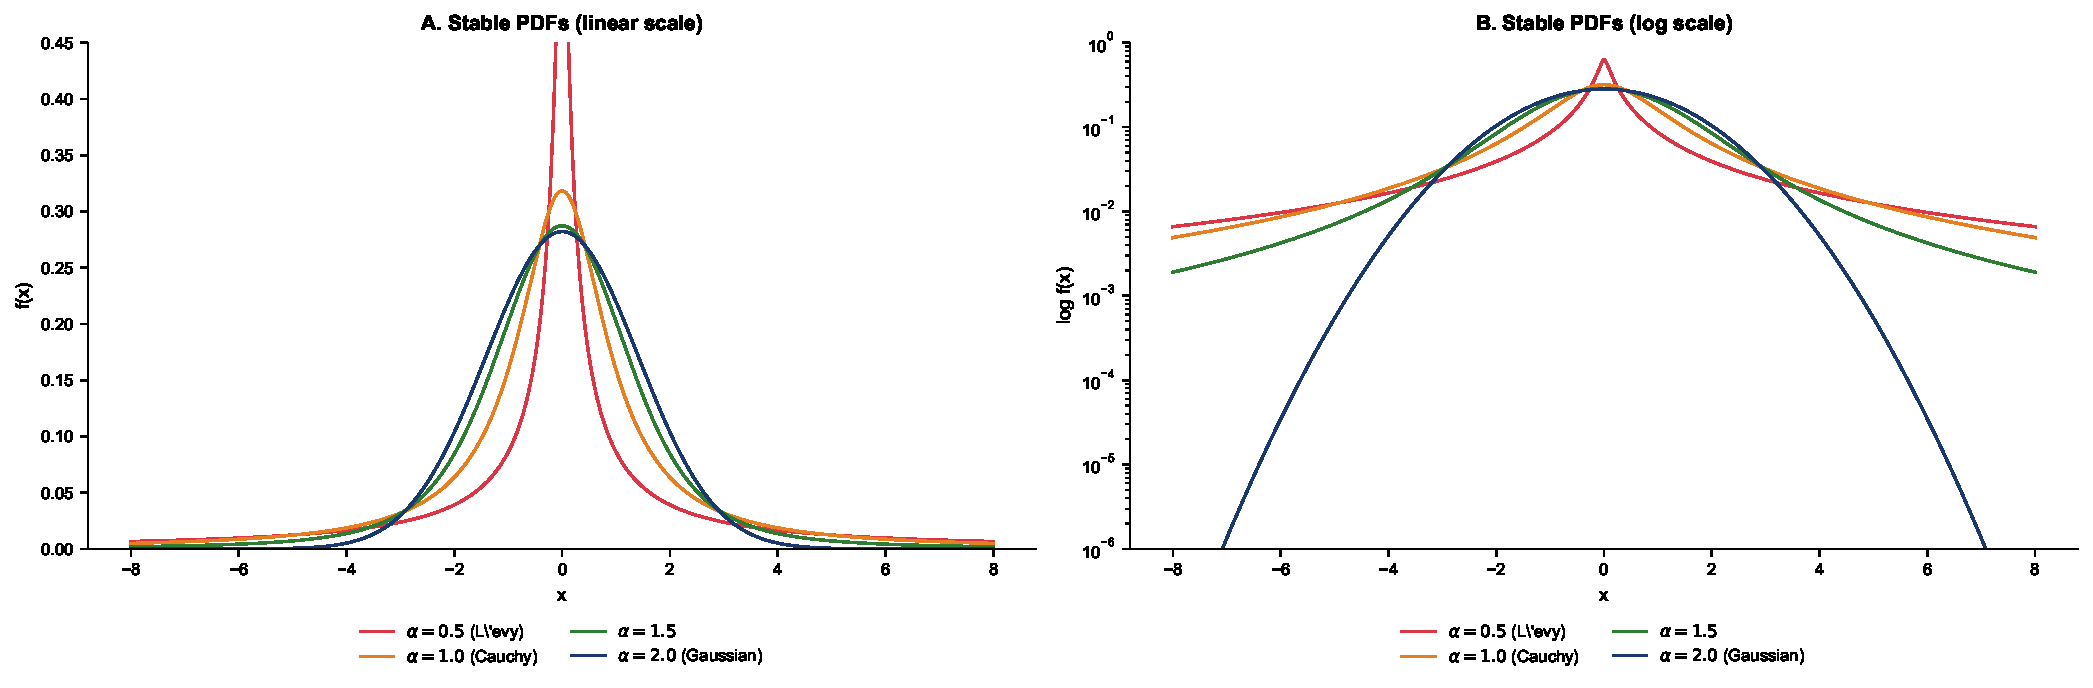
\includegraphics[width=\textwidth]{ch2_stable_pdfs.pdf}
            {\tiny Familii stabile: de la Lévy la Gaussiană}
        \end{column}
    \end{columns}
\end{cminipage}
\end{frame}

\begin{frame}{Spectrul Distribuțiilor Stabile: $\alpha$ de la 0 la 2}
\begin{cminipage}{0.95\textwidth}
    \begin{center}
    \begin{tikzpicture}[
        x=5.5cm, y=0.5cm,
        every node/.style={font=\footnotesize}
    ]
    % Axis
    \draw[-{Stealth}, thick] (0,0) -- (2.3,0) node[right] {$\alpha$};
    % Ticks
    \foreach \x/\lab in {0.25/0.5, 0.5/1.0, 0.75/1.5, 1.0/2.0} {
        \draw (\x,-0.2) -- (\x,0.2) node[above=3pt] {\lab};
    }
    % Labels below
    \node[below=8pt] at (0.25,0) {Lévy};
    \node[below=8pt] at (0.5,0) {Cauchy};
    \node[below=8pt, text=MainBlue] at (0.75,0) {\textbf{Finanțe}};
    \node[below=8pt] at (1.0,0) {Normal};
    % Bracket for finance
    \draw[MainBlue, thick, decorate, decoration={brace, amplitude=5pt, mirror}]
        (0.62,-1.5) -- (0.92,-1.5) node[midway, below=5pt] {\scriptsize $\alpha \in [1.5, 1.9]$};
    % Arrows with properties
    \draw[Crimson, ->, thick] (0.15,2) -- (0.15,0.5);
    \node[above, Crimson] at (0.15,2) {\scriptsize Cozi foarte grele};
    \draw[Forest, ->, thick] (1.05,2) -- (1.05,0.5);
    \node[above, Forest] at (1.05,2) {\scriptsize Cozi exponențiale};
    \end{tikzpicture}
    \end{center}

    \vspace{0.3cm}
    \begin{itemize}\setlength{\itemsep}{0pt}
        \item $\alpha \to 0$: cozi din ce în ce mai grele, toate momentele divergente
        \item $\alpha = 2$: distribuția normală (cozi exponențiale, toate momentele finite)
        \item \textbf{Randamente financiare:} $\hat{\alpha} \in [1.5, 1.9]$ --- între Cauchy și Normal
        \item $\alpha$ mai mic $\Rightarrow$ evenimente ``lebădă neagră'' mai frecvente
    \end{itemize}
\end{cminipage}
\end{frame}

%=============================================================================
% PARTEA I: EXERCIȚII MANUAL
%=============================================================================
\section{Partea I: Exerciții manual}

\begin{frame}{Exercițiul 1: Verificarea stabilității --- Cazul Gaussian}
    \begin{cminipage}{0.95\textwidth}
\begin{block}{Problemă}
\begin{itemize}\setlength{\itemsep}{0pt}
    \item Fie $X_1, X_2$ variabile i.i.d. $\sim \mathcal{N}(0, 1)$. Arătați că
$a X_1 + b X_2 \stackrel{d}{=} c X + d$ pentru $a=3, b=4, c=5$.
\end{itemize}
\end{block}

\begin{exampleblock}{Rezolvare}
\begin{itemize}\setlength{\itemsep}{0pt}
    \item Dacă $X_1 \sim \mathcal{N}(0, 1)$, atunci $aX_1 \sim \mathcal{N}(0, a^2)$ și $bX_2 \sim \mathcal{N}(0, b^2)$.
    \item Suma: $aX_1 + bX_2 \sim \mathcal{N}(0, a^2 + b^2) = \mathcal{N}(0, 9 + 16) = \mathcal{N}(0, 25)$.
    \item Deci $c = \sqrt{a^2 + b^2} = \sqrt{25} = 5$ și $d = 0$.
    \item \textbf{Concluzie:} Distribuția normală este stabilă cu $\alpha = 2$. Proprietatea de stabilitate se reduce la regula adunării varianțelor.
\end{itemize}
\end{exampleblock}
    \end{cminipage}
\end{frame}

\begin{frame}{Exercițiul 1 cont.: Cazul Cauchy + Tabel comparativ}
    \begin{cminipage}{0.95\textwidth}
\begin{columns}[T]
\begin{column}{0.48\textwidth}
\begin{block}{Cazul Cauchy ($\alpha = 1$)}
\begin{itemize}\setlength{\itemsep}{0pt}
    \item Fie $X_1, X_2 \sim \text{Cauchy}(0,1)$ i.i.d.
    \item $aX_1 + bX_2 \sim \text{Cauchy}(0, a+b)$
    \item Pentru $a=3, b=4$: $c = a + b = 7$, $d = 0$.
    \item \textbf{Notă:} La Cauchy, scara se adună \textit{liniar}, nu pătratic!
\end{itemize}
\end{block}
\end{column}
\begin{column}{0.48\textwidth}
\begin{block}{Regula generală}
\begin{itemize}\setlength{\itemsep}{0pt}
    \item Pentru $S(\alpha, \beta, \gamma, \delta)$:
$$c^\alpha = a^\alpha + b^\alpha$$
\end{itemize}

\vspace{0.2cm}
\renewcommand{\arraystretch}{1.3}
\begin{tabular}{lccc}
\toprule
& $\alpha$ & Regulă & $c$ \\
\midrule
Gaussian & 2 & $c^2 = a^2+b^2$ & 5 \\
Cauchy & 1 & $c = a+b$ & 7 \\
$S(1.5)$ & 1.5 & $c^{1.5} = a^{1.5}+b^{1.5}$ & 6.19 \\
\bottomrule
\end{tabular}
\end{block}
\end{column}
\end{columns}
    \end{cminipage}
\end{frame}

\begin{frame}{Exercițiul 2: Funcția caracteristică}
    \begin{cminipage}{0.95\textwidth}
\begin{block}{Problemă}
\begin{itemize}\setlength{\itemsep}{0pt}
    \item Calculați $\varphi_X(t)$ pentru $X \sim S(1.5, 0.3, 1, 0)$ la $t = 1$.
\end{itemize}
\end{block}

\begin{exampleblock}{Rezolvare}
\begin{itemize}\setlength{\itemsep}{0pt}
    \item Funcția caracteristică a distribuției stabile:
$$\log \varphi_X(t) = -|t|^\alpha \left[1 - i\beta\,\text{sgn}(t)\tan\frac{\pi\alpha}{2}\right] + i\delta t$$
    \item Pentru $\alpha = 1.5$, $\beta = 0.3$, $\gamma = 1$, $\delta = 0$, $t = 1$:
$$\log \varphi_X(1) = -|1|^{1.5}\left[1 - i \cdot 0.3 \cdot 1 \cdot \tan\frac{3\pi}{4}\right]$$
$$= -1 \cdot [1 - i \cdot 0.3 \cdot (-1)] = -1 - 0.3i$$
    \item Deci:
$$\varphi_X(1) = e^{-1 - 0.3i} = e^{-1}(\cos 0.3 - i\sin 0.3) \approx 0.351 - 0.109i$$
$$|\varphi_X(1)| = e^{-1} \approx 0.368$$
\end{itemize}
\end{exampleblock}
    \end{cminipage}
\end{frame}

\begin{frame}{Exercițiul 3: Momente și cozi}
    \begin{cminipage}{0.95\textwidth}
\begin{block}{Problemă}
\begin{itemize}\setlength{\itemsep}{0pt}
    \item Un analist financiar modelează randamentele zilnice cu $S(1.7, -0.2, 0.01, 0.0005)$. Care momente există? Ce implică pentru managementul riscului?
\end{itemize}
\end{block}

\begin{exampleblock}{Rezolvare}
\begin{columns}[T]
\begin{column}{0.48\textwidth}
\begin{itemize}\setlength{\itemsep}{0pt}
    \item \textbf{Existența momentelor:}
    \item $\E[|X|^p] < \infty$ dacă și numai dacă $p < \alpha$
    \item $\alpha = 1.7 \Rightarrow$
    \begin{itemize}\setlength{\itemsep}{0pt}
        \item Media ($p=1$): \textcolor{Forest}{există} ($1 < 1.7$)
        \item Varianța ($p=2$): \textcolor{Crimson}{nu există} ($2 > 1.7$)
        \item Kurtosis ($p=4$): \textcolor{Crimson}{nu există}
    \end{itemize}
\end{itemize}
\end{column}
\begin{column}{0.48\textwidth}
\begin{itemize}\setlength{\itemsep}{0pt}
    \item \textbf{Implicații practice:}
    \item $\beta = -0.2$: asimetrie negativă (risc la căderi)
    \item VaR Gaussian \textbf{subestimează} riscul real
    \item Probabilitatea unui eveniment $-5\sigma$:
    \begin{itemize}\setlength{\itemsep}{0pt}
        \item Normal: $\approx 3 \times 10^{-7}$ (1 la 3.5M zile)
        \item Stabil(1.7): $\approx 0.003$ (1 la 333 zile)
    \end{itemize}
    \item Sharpe ratio nu este definit riguros!
\end{itemize}
\end{column}
\end{columns}
\end{exampleblock}
    \end{cminipage}
\end{frame}

\begin{frame}{Exercițiul 3b: Verificarea stabilității pentru $\alpha = 1.5$}
    \begin{cminipage}{0.95\textwidth}
\begin{block}{Problemă}
\begin{itemize}\setlength{\itemsep}{0pt}
    \item Fie $X_1, X_2 \sim S(1.5, 0, 1, 0)$ i.i.d. Calculați constanta $c$ astfel încât $X_1 + X_2 \sim S(1.5, 0, c, 0)$, pentru $a = b = 1$.
\end{itemize}
\end{block}

\begin{exampleblock}{Rezolvare}
\begin{itemize}\setlength{\itemsep}{0pt}
    \item \textbf{Formula:} $c^\alpha = a^\alpha + b^\alpha$
    \item $c^{1.5} = 1^{1.5} + 1^{1.5} = 2$
    \item $c = 2^{1/1.5} = 2^{2/3} \approx \mathbf{1.587}$
\end{itemize}

\vspace{0.2cm}
\begin{itemize}\setlength{\itemsep}{0pt}
    \item \textbf{Comparație cu Normal ($\alpha = 2$):}
    \item Normal: $c = 2^{1/2} = \sqrt{2} \approx 1.414$
    \item Stabil(1.5): $c = 2^{2/3} \approx 1.587$
    \item $\Rightarrow$ Suma a două variabile stabile crește scara \textbf{mai repede} decât sub Normal
    \item Implicație: diversificarea reduce riscul \textbf{mai puțin eficient} sub distribuții stabile
\end{itemize}
\end{exampleblock}
    \end{cminipage}
\end{frame}

\begin{frame}{Exercițiul 3c: Densitatea stabilă vs normală în puncte cheie}
    \begin{cminipage}{0.95\textwidth}
\begin{block}{Problemă}
\begin{itemize}\setlength{\itemsep}{0pt}
    \item Comparați $P(|X| > k)$ pentru Normal vs $S(1.7, 0, 1, 0)$, pentru $k = 2, 3, 5$.
\end{itemize}
\end{block}

\begin{exampleblock}{Rezolvare}
\renewcommand{\arraystretch}{1.3}
\begin{center}
\begin{tabular}{lcccc}
\toprule
$k$ & $P_{\text{Normal}}(|X|>k)$ & $P_{\text{Stabil}}(|X|>k)$ & \textbf{Raport} & \textbf{Frecvență stabil} \\
\midrule
2 & 4.56\% & 8.2\% & 1.8$\times$ & 1 la 12 zile \\
3 & 0.27\% & 2.1\% & 7.8$\times$ & 1 la 48 zile \\
5 & 0.000057\% & 0.35\% & 6{,}100$\times$ & 1 la 286 zile \\
\bottomrule
\end{tabular}
\end{center}

\begin{itemize}\setlength{\itemsep}{0pt}
    \item Diferența crește \textbf{dramatic} cu $k$
    \item La $k = 5$: evenimentul este de 6{,}100$\times$ mai probabil sub modelul stabil
    \item $\Rightarrow$ Modelul normal \textbf{subestimează} frecvența evenimentelor extreme
\end{itemize}
\end{exampleblock}
    \end{cminipage}
\end{frame}

%=============================================================================
% PARTEA II: ESTIMARE
%=============================================================================
\section{Partea II: Estimare}

\begin{frame}{Metoda McCulloch --- Concept}
    \begin{cminipage}{0.95\textwidth}
\begin{block}{Ideea principală}
\begin{itemize}\setlength{\itemsep}{0pt}
    \item Estimarea parametrilor $(\alpha, \beta, \gamma, \delta)$ din \textbf{cuantile} ale eșantionului.
\end{itemize}
\end{block}

\begin{columns}[T]
\begin{column}{0.48\textwidth}
\begin{itemize}\setlength{\itemsep}{0pt}
    \item \textbf{Statistici intermediare:}
\end{itemize}
$$v_\alpha = \frac{q_{0.95} - q_{0.05}}{q_{0.75} - q_{0.25}}$$
$$v_\beta = \frac{q_{0.95} + q_{0.05} - 2q_{0.50}}{q_{0.95} - q_{0.05}}$$

\vspace{0.2cm}
\begin{itemize}\setlength{\itemsep}{0pt}
    \item $v_\alpha$ măsoară \textit{greutatea cozilor} (tail thickness)
    \item $v_\beta$ măsoară \textit{asimetria}
\end{itemize}
\end{column}
\begin{column}{0.48\textwidth}
\begin{itemize}\setlength{\itemsep}{0pt}
    \item \textbf{Tabel de referință (selecție):}
\end{itemize}

\renewcommand{\arraystretch}{1.2}
\begin{tabular}{ccc}
\toprule
$v_\alpha$ & $\alpha$ & Interpretare \\
\midrule
2.44 & 2.0 & Gaussiană \\
2.62 & 1.9 & Aproape Gauss \\
3.04 & 1.7 & Cozi moderate \\
4.21 & 1.5 & Cozi grele \\
6.31 & 1.3 & Cozi foarte grele \\
\bottomrule
\end{tabular}
\end{column}
\end{columns}
    \end{cminipage}
\end{frame}

\begin{frame}{McCulloch --- Exercițiu rezolvat}
    \begin{cminipage}{0.95\textwidth}
\begin{block}{Date numerice}
\begin{itemize}\setlength{\itemsep}{0pt}
    \item Din eșantionul de 2000 observații: $q_{0.05} = -3.42$, $q_{0.25} = -0.78$, $q_{0.50} = 0.05$, $q_{0.75} = 0.82$, $q_{0.95} = 3.61$.
\end{itemize}
\end{block}

\begin{exampleblock}{Rezolvare pas cu pas}
\begin{itemize}\setlength{\itemsep}{0pt}
    \item \textbf{Pasul 1: Calculăm $v_\alpha$}
$$v_\alpha = \frac{q_{0.95} - q_{0.05}}{q_{0.75} - q_{0.25}} = \frac{3.61 - (-3.42)}{0.82 - (-0.78)} = \frac{7.03}{1.60} = 4.39$$
    \item \textbf{Pasul 2: Estimăm $\alpha$} --- Din tabel: $v_\alpha = 4.39$ corespunde $\hat{\alpha} \approx 1.48$.
    \item \textbf{Pasul 3: Calculăm $v_\beta$}
$$v_\beta = \frac{q_{0.95} + q_{0.05} - 2q_{0.50}}{q_{0.95} - q_{0.05}} = \frac{3.61 + (-3.42) - 2 \cdot 0.05}{7.03} = \frac{0.09}{7.03} \approx 0.013$$
    \item \textbf{Pasul 4: Estimăm $\beta$} --- $v_\beta \approx 0.013 \approx 0 \Rightarrow \hat{\beta} \approx 0$ (distribuție aproape simetrică).
\end{itemize}
\end{exampleblock}
    \end{cminipage}
\end{frame}

\begin{frame}[fragile]{Maximum Likelihood Estimation (MLE)}
\begin{block}{Procedura}
$$\hat{\theta}_{MLE} = \arg\max_{\theta} \sum_{i=1}^{n} \log f(x_i; \alpha, \beta, \gamma, \delta)$$
\end{block}

\begin{columns}[T]
\begin{column}{0.48\textwidth}
\begin{itemize}\setlength{\itemsep}{0pt}
    \item \textbf{Provocări:}
    \item PDF-ul nu are formă închisă (în general)
    \item Trebuie evaluare numerică prin FFT
    \item Funcția de verosimilitate nu e convexă
    \item Convergență lentă pentru $\alpha$ mic
\end{itemize}
\end{column}
\begin{column}{0.48\textwidth}
\begin{itemize}\setlength{\itemsep}{0pt}
    \item \textbf{Avantaje:}
    \item Cea mai eficientă estimare asimptotic
    \item Intervale de încredere standard
    \item Implementare modernă: \texttt{scipy.stats.levy\_stable.fit()}
\end{itemize}

\vspace{0.2cm}
\begin{itemize}\setlength{\itemsep}{0pt}
    \item \textbf{One-liner Python:}
\end{itemize}
\begin{lstlisting}
from scipy.stats import levy_stable
a, b, loc, sc = levy_stable.fit(data)
\end{lstlisting}
\end{column}
\end{columns}
\end{frame}

\begin{frame}{Regresia Koutrouvelis}
    \begin{cminipage}{0.95\textwidth}
\begin{block}{Metoda în 2 etape}
\begin{itemize}\setlength{\itemsep}{0pt}
    \item Se utilizează funcția caracteristică empirică (ECF).
\end{itemize}
\end{block}

\begin{itemize}\setlength{\itemsep}{0pt}
    \item \textbf{Etapa 1:} Estimarea $\alpha$ și $\gamma$ prin regresie liniară:
$$\log\left(-\log|\hat{\varphi}_n(t)|^2\right) = \log(2\gamma^\alpha) + \alpha \log|t|$$
    \item Regresie $Y = a + bX$ cu $Y_k = \log(-\log|\hat{\varphi}_n(t_k)|^2)$ și $X_k = \log|t_k|$.
    \item \textbf{Etapa 2:} Estimarea $\beta$ și $\delta$ prin regresie pe partea imaginară:
$$\arg[\hat{\varphi}_n(t)] = \delta t - \beta\gamma^\alpha \tan\frac{\pi\alpha}{2}\,\text{sgn}(t)|t|^\alpha$$
\end{itemize}

\begin{alertblock}{Avantaj}
\begin{itemize}\setlength{\itemsep}{0pt}
    \item Robustă numeric, nu necesită evaluarea PDF-ului, convergență rapidă.
\end{itemize}
\end{alertblock}
    \end{cminipage}
\end{frame}

\begin{frame}{Comparație: McCulloch vs MLE vs Koutrouvelis}
    \begin{cminipage}{0.95\textwidth}
\begin{itemize}\setlength{\itemsep}{0pt}
    \item \textbf{Problemă:} Pe $n = 5000$ randamente zilnice S\&P 500, cele 3 metode dau:
\end{itemize}

\vspace{0.2cm}
\renewcommand{\arraystretch}{1.3}
\begin{center}
\begin{tabular}{lcccc}
\toprule
\textbf{Metodă} & $\hat{\alpha}$ & $\hat{\beta}$ & $\hat{\gamma}$ & \textbf{Timp calcul} \\
\midrule
McCulloch & 1.72 & $-0.15$ & 0.0083 & $< 0.01$s \\
Koutrouvelis & 1.69 & $-0.19$ & 0.0081 & $\sim 0.1$s \\
MLE & 1.71 & $-0.18$ & 0.0082 & $\sim 30$s \\
\bottomrule
\end{tabular}
\end{center}

\begin{itemize}\setlength{\itemsep}{0pt}
    \item \textbf{Observații:}
    \item Toate metodele dau $\hat{\alpha} \approx 1.7$ --- consistent
    \item McCulloch: cel mai rapid, dar mai puțin precis (bazat pe doar 5 cuantile)
    \item MLE: cel mai precis asimptotic, dar \textbf{foarte lent}
    \item Koutrouvelis: compromis bun viteză/precizie
    \item \textbf{Recomandare:} McCulloch pentru explorare rapidă, MLE pentru rapoarte finale
\end{itemize}
    \end{cminipage}
\end{frame}

%=============================================================================
% PARTEA III: COZI ȘI RISC
%=============================================================================
\section{Partea III: Cozi și risc}

\begin{frame}{Heavy tails --- Gaussiană vs Stabilă}
    \begin{cminipage}{0.95\textwidth}
\quantlet{SFM\_ch2\_stable\_fit}{https://github.com/QuantLet/Stat_fin_markets/tree/master/Ch_02/SFM_ch2_stable_distributions}

\begin{block}{Tabel comparativ: Probabilitatea evenimentelor extreme}
\renewcommand{\arraystretch}{1.3}
\begin{center}
\begin{tabular}{lccc}
\toprule
\textbf{Eveniment} & \textbf{Gaussiană} & \textbf{Stabil($\alpha$=1.7)} & \textbf{Raport} \\
\midrule
$|X| > 3\sigma$ & $2.7 \times 10^{-3}$ & $1.9 \times 10^{-2}$ & $\approx 7\times$ \\
$|X| > 5\sigma$ & $5.7 \times 10^{-7}$ & $3.0 \times 10^{-3}$ & $\approx 5{,}000\times$ \\
$|X| > 10\sigma$ & $1.5 \times 10^{-23}$ & $5.2 \times 10^{-4}$ & $\approx 10^{19}\times$ \\
\bottomrule
\end{tabular}
\end{center}
\end{block}

\begin{alertblock}{Implicație practică}
\begin{itemize}\setlength{\itemsep}{0pt}
    \item Modelele Gaussiene subestimează dramatic riscul evenimentelor extreme. Un eveniment ``$10\sigma$'' pe care Gaussiana îl consideră practic imposibil apare o dată la $\sim$2{,}000 de zile ($\sim$8 ani) sub modelul stabil.
\end{itemize}
\end{alertblock}
    \end{cminipage}
\end{frame}

\begin{frame}{Exercițiul 4: VaR Gaussiană vs Stabilă}
    \begin{cminipage}{0.95\textwidth}
\begin{block}{Problemă}
\begin{itemize}\setlength{\itemsep}{0pt}
    \item Portofoliu de 1{,}000{,}000 EUR. Randamente zilnice modelate cu $S(1.7, -0.2, 0.01, 0.0005)$. Comparați VaR la 1\%, 5\% și 0.1\%.
\end{itemize}
\end{block}

\begin{exampleblock}{Rezolvare}
\renewcommand{\arraystretch}{1.3}
\begin{center}
\begin{tabular}{lccc}
\toprule
\textbf{Nivel VaR} & \textbf{Gaussiană} & \textbf{Stabilă} & \textbf{Diferență} \\
\midrule
5\% & $-$16{,}449 EUR & $-$21{,}340 EUR & +30\% \\
1\% & $-$22{,}763 EUR & $-$39{,}870 EUR & +75\% \\
0.1\% & $-$30{,}091 EUR & $-$87{,}420 EUR & +190\% \\
\bottomrule
\end{tabular}
\end{center}

\begin{itemize}\setlength{\itemsep}{0pt}
    \item \textbf{Concluzie:} Cu cât nivelul de încredere este mai mare (cozi mai adânci), cu atât diferența Gaussiană vs Stabilă crește. La VaR 0.1\%, modelul stabil estimează pierderi de aproape \textbf{3 ori mai mari}.
\end{itemize}
\end{exampleblock}
    \end{cminipage}
\end{frame}

\begin{frame}{Comparație vizuală: Funcția de supraviețuire}
    \begin{cminipage}{0.95\textwidth}
\quantlet{SFM\_ch2\_stable\_fit}{https://github.com/QuantLet/Stat_fin_markets/tree/master/Ch_02/SFM_ch2_stable_distributions}

\begin{center}
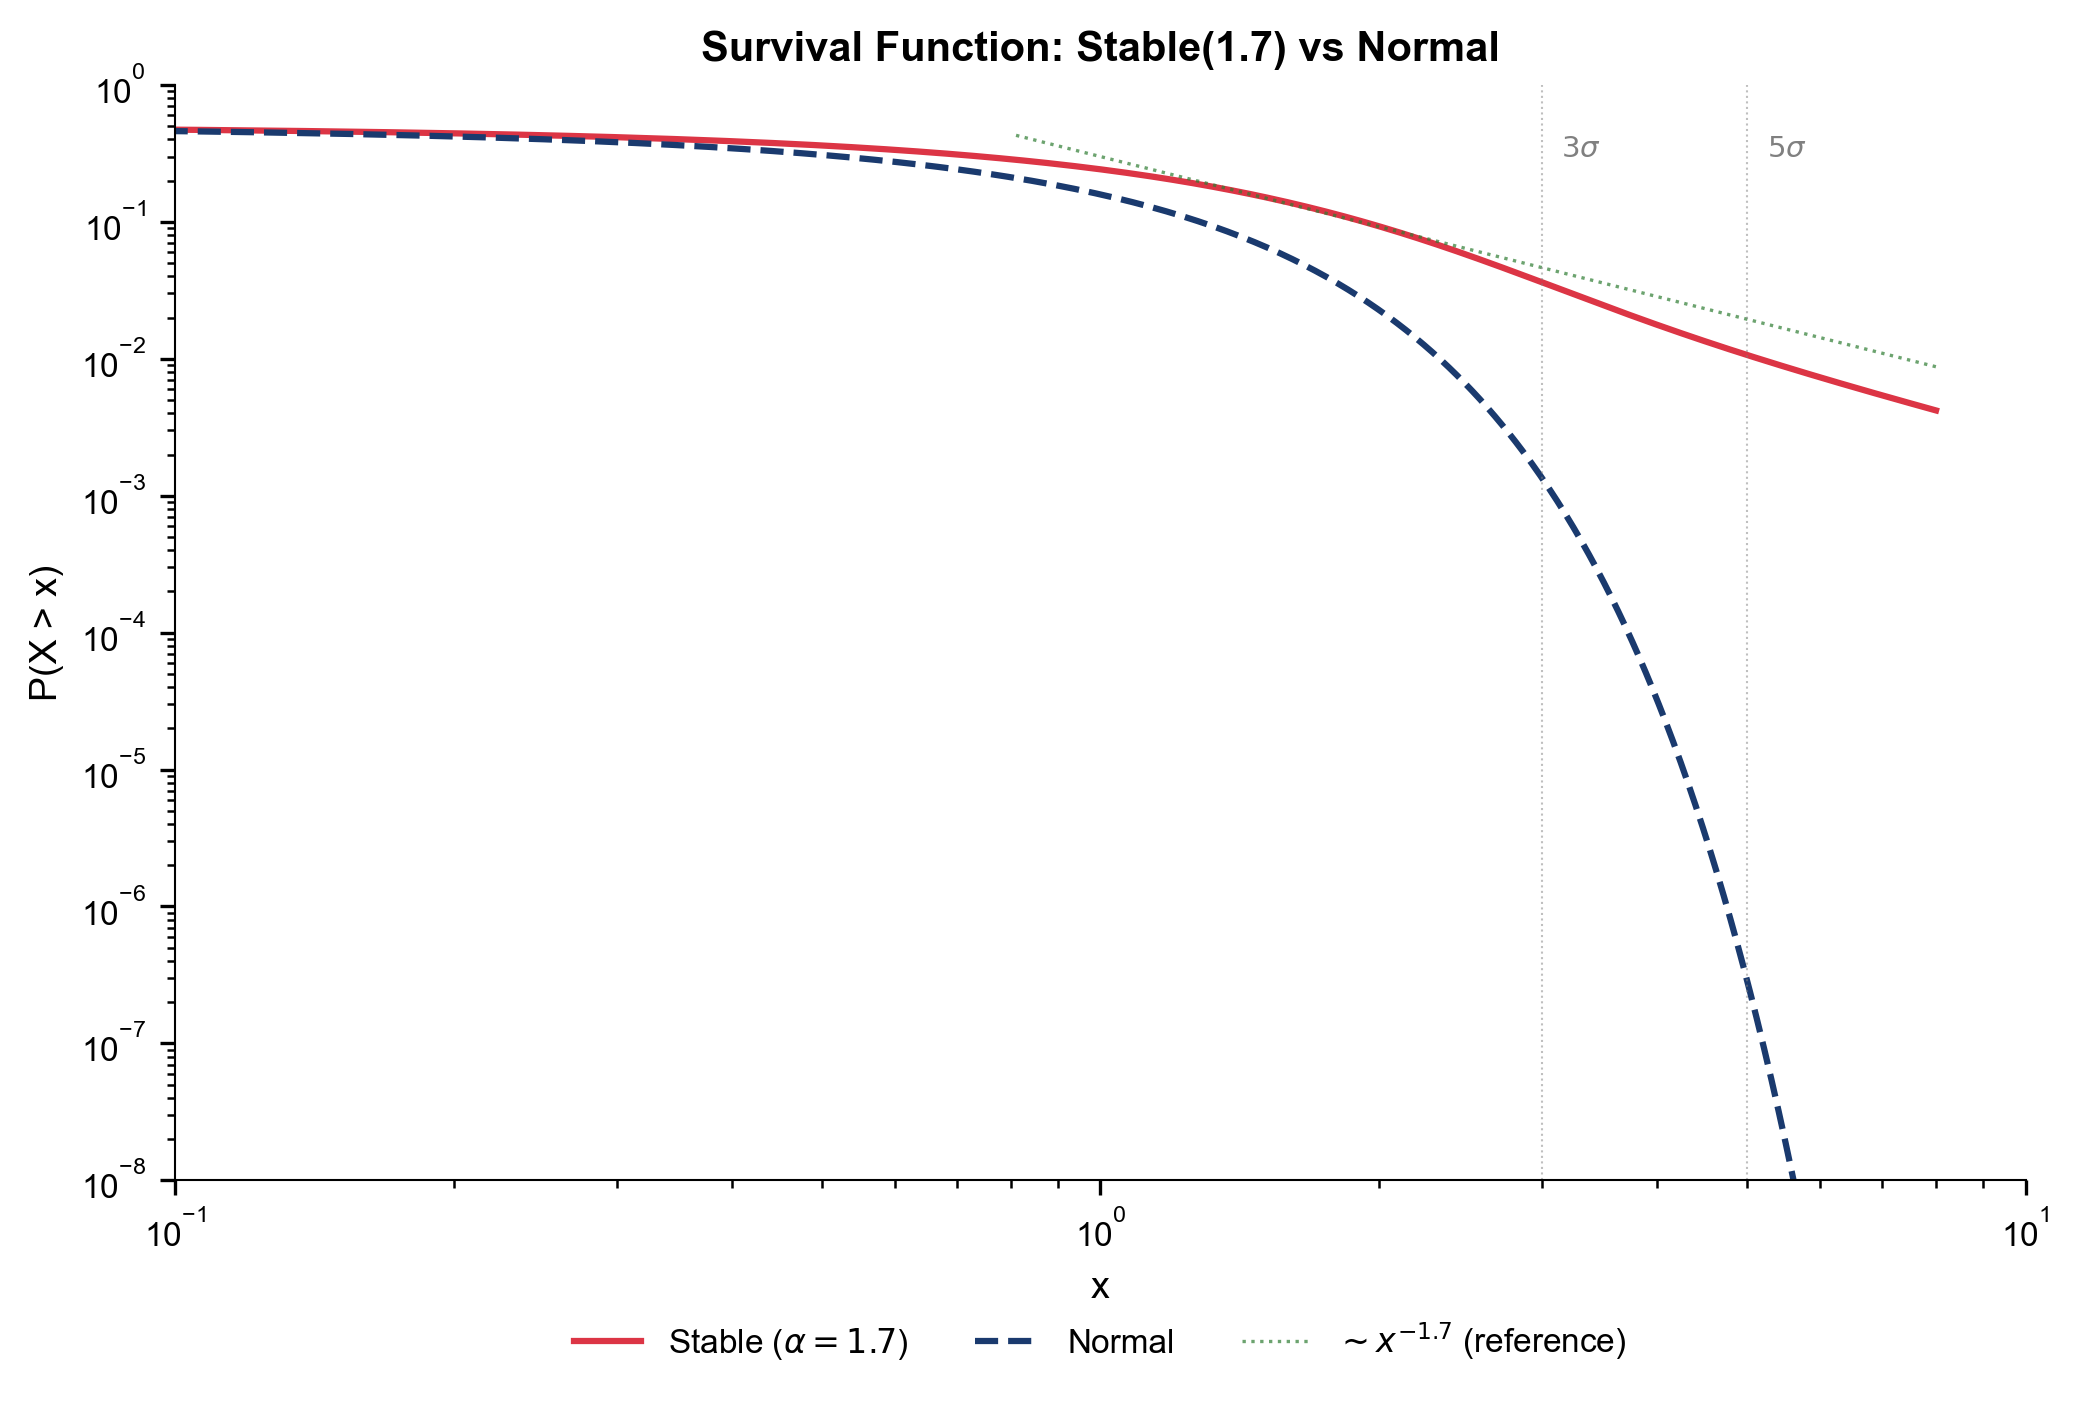
\includegraphics[width=0.75\textwidth]{ch2_tail_survival.png}
\end{center}

\vspace{-0.3cm}
\begin{itemize}\setlength{\itemsep}{0pt}
    \item Grafic log-log: funcția de supraviețuire $P(X > x)$
    \item Distribuția stabilă scade ca o \textbf{lege putere}: $P(X > x) \sim C_\alpha x^{-\alpha}$
    \item Distribuția normală scade \textbf{exponențial}: diferența crește rapid cu $x$
\end{itemize}
    \end{cminipage}
\end{frame}

\begin{frame}{Exercițiul 5: Expected Shortfall sub Distribuție Stabilă}
    \begin{cminipage}{0.95\textwidth}
\begin{block}{Problemă}
\begin{itemize}\setlength{\itemsep}{0pt}
    \item Portofoliu de 1{,}000{,}000 EUR. Randamente $\sim S(1.7, -0.2, 0.01, 0)$.
    \item Calculați raportul ES/VaR la 1\% și comparați cu cazul Normal.
\end{itemize}
\end{block}

\begin{exampleblock}{Rezolvare}
\begin{columns}[T]
\begin{column}{0.48\textwidth}
\begin{itemize}\setlength{\itemsep}{0pt}
    \item \textbf{Normal:}
    \item VaR$_{1\%}$ = 22{,}763 EUR
    \item ES$_{1\%}$ = 26{,}152 EUR
    \item ES/VaR = \textbf{1.149}
\end{itemize}
\end{column}
\begin{column}{0.48\textwidth}
\begin{itemize}\setlength{\itemsep}{0pt}
    \item \textbf{Stabil ($\alpha = 1.7$):}
    \item VaR$_{1\%}$ = 39{,}870 EUR
    \item ES$_{1\%}$ = 67{,}779 EUR
    \item ES/VaR = \textbf{1.700}
\end{itemize}
\end{column}
\end{columns}

\vspace{0.2cm}
\begin{itemize}\setlength{\itemsep}{0pt}
    \item $\Rightarrow$ Sub distribuția stabilă, ES este cu \textbf{70\%} mai mare decât VaR (vs 15\% sub Normal)
    \item Motiv: cozile grele contribuie enorm la media pierderilor condiționate
    \item \textbf{Regulă practică:} ES/VaR crește cu scăderea lui $\alpha$
\end{itemize}
\end{exampleblock}
    \end{cminipage}
\end{frame}

\begin{frame}{Exercițiul 6: Backtesting VaR --- Câte depășiri?}
    \begin{cminipage}{0.95\textwidth}
\begin{block}{Problemă}
\begin{itemize}\setlength{\itemsep}{0pt}
    \item Pe 2500 de zile de tranzacționare ($\approx$ 10 ani), VaR la 1\% a fost depășit de:
\end{itemize}
\end{block}

\vspace{0.1cm}
\renewcommand{\arraystretch}{1.3}
\begin{center}
\begin{tabular}{lccc}
\toprule
\textbf{Model} & \textbf{Depășiri așteptate} & \textbf{Depășiri observate} & \textbf{Verdict} \\
\midrule
Normal & 25 (1\%) & 58 & \textcolor{Crimson}{\textbf{Subestimează}} \\
Stabil($\alpha = 1.7$) & 25 (1\%) & 29 & \textcolor{Forest}{\textbf{Bun}} \\
Empiric & 25 (1\%) & 25 & \textcolor{Forest}{\textbf{Exact}} \\
\bottomrule
\end{tabular}
\end{center}

\begin{itemize}\setlength{\itemsep}{0pt}
    \item Normalul: 58 depășiri vs 25 așteptate $\Rightarrow$ \textbf{2.3$\times$} mai multe
    \item Modelul stabil: aproape de numărul așteptat
    \item \textbf{Testul Kupiec (LR):} compară proporția observată cu cea așteptată
    \item $LR = 2\left[v\ln\frac{v/n}{\alpha} + (n-v)\ln\frac{1-v/n}{1-\alpha}\right] \sim \chi^2(1)$
\end{itemize}
    \end{cminipage}
\end{frame}

\begin{frame}{Adevărat sau Fals? --- Distribuții Stabile}
\begin{cminipage}{0.95\textwidth}
    \begin{itemize}\setlength{\itemsep}{0pt}
        \item \textbf{Răspundeți cu Adevărat (A) sau Fals (F):}
    \end{itemize}
    \vspace{0.2cm}
    \footnotesize
    \begin{enumerate}\setlength{\itemsep}{1pt}
        \item Distribuția normală este un caz special al distribuțiilor stabile (cu $\alpha = 2$).
        \item Distribuția Cauchy ($\alpha = 1$) are medie finită.
        \item Dacă $\alpha = 1.8$, varianța eșantionului $s^2$ converge la o constantă finită pe măsură ce $n \to \infty$.
        \item Funcția caracteristică a unei distribuții stabile are întotdeauna formă închisă.
        \item Metoda McCulloch este mai eficientă asimptotic decât MLE.
        \item Cozile distribuției stabile scad ca o lege putere $x^{-\alpha}$.
        \item VaR-ul sub distribuția stabilă este întotdeauna mai mare decât sub normală.
    \end{enumerate}
    \normalsize
    \vspace{0.2cm}
    \begin{exampleblock}{Răspunsuri}
    \footnotesize
    \begin{enumerate}\setlength{\itemsep}{1pt}
        \item \textcolor{Forest}{\textbf{A}}: Normal $\equiv S(2, 0, \sigma/\sqrt{2}, \mu)$
        \item \textcolor{Crimson}{\textbf{F}}: Cauchy nu are niciun moment finit (nici media!)
        \item \textcolor{Crimson}{\textbf{F}}: Cu $\alpha = 1.8 < 2$, varianța teoretică este $\infty$; $s^2$ \textbf{diverge}
        \item \textcolor{Forest}{\textbf{A}}: $\log\varphi(t)$ are formă parametrică; dar PDF-ul \textbf{nu} are formă închisă
        \item \textcolor{Crimson}{\textbf{F}}: MLE este cea mai eficientă; McCulloch este rapidă dar sub-optimală
        \item \textcolor{Forest}{\textbf{A}}: $P(X > x) \sim C_\alpha x^{-\alpha}$ (comportament paretian)
        \item \textcolor{Crimson}{\textbf{F}}: La 5\%, diferența este mică; la 0.1\% însă, diferența este enormă
    \end{enumerate}
    \end{exampleblock}
\end{cminipage}
\end{frame}

%=============================================================================
% PARTEA IV: PYTHON
%=============================================================================
\section{Partea IV: Implementare Python}

\begin{frame}[fragile]{Simulare: Stable Distributions}
\begin{lstlisting}
import numpy as np
from scipy.stats import levy_stable
import matplotlib.pyplot as plt

alphas = [0.5, 1.0, 1.5, 2.0]
x = np.linspace(-8, 8, 1000)

fig, (ax1, ax2) = plt.subplots(1, 2, figsize=(14, 5))
colors = ['#DC3545', '#FF8C00', '#2E7D32', '#1A3A6E']
labels = ['alpha=0.5 (Levy)', 'alpha=1.0 (Cauchy)',
          'alpha=1.5', 'alpha=2.0 (Gaussian)']

for a, c, lab in zip(alphas, colors, labels):
    pdf = levy_stable.pdf(x, alpha=a, beta=0)
    ax1.plot(x, pdf, color=c, label=lab)
    ax2.semilogy(x, pdf, color=c, label=lab)

ax1.set_title('PDFs (linear)')
ax2.set_title('PDFs (log scale)')
for ax in [ax1, ax2]:
    ax.legend(loc='upper center',
              bbox_to_anchor=(0.5, -0.12), ncol=2)
plt.tight_layout()
\end{lstlisting}
\end{frame}

\begin{frame}[fragile]{Python: Stable Fit S\&P 500}
\begin{lstlisting}
import yfinance as yf
from scipy.stats import levy_stable, norm

sp500 = yf.download('^GSPC', start='2000-01-01',
                     end='2025-12-31')
returns = np.log(
    sp500['Close'] / sp500['Close'].shift(1)).dropna()

# Fit stable distribution
alpha, beta, loc, scale = levy_stable.fit(returns.values)
print(f"alpha={alpha:.3f}, beta={beta:.3f}")

# Fit normal
mu, sigma = norm.fit(returns.values)

# Compare on log-scale
x = np.linspace(returns.min()*1.2,
                returns.max()*1.2, 1000)
plt.hist(returns, bins=150, density=True,
         alpha=0.4, label='Data')
plt.semilogy(x, levy_stable.pdf(x, alpha, beta,
             loc, scale), label='Stable')
plt.semilogy(x, norm.pdf(x, mu, sigma),
             '--', label='Normal')
\end{lstlisting}
\end{frame}

\begin{frame}{Overlay PDF: Histogram + Stable + Normal (log-scale)}
    \begin{cminipage}{0.95\textwidth}
\begin{center}
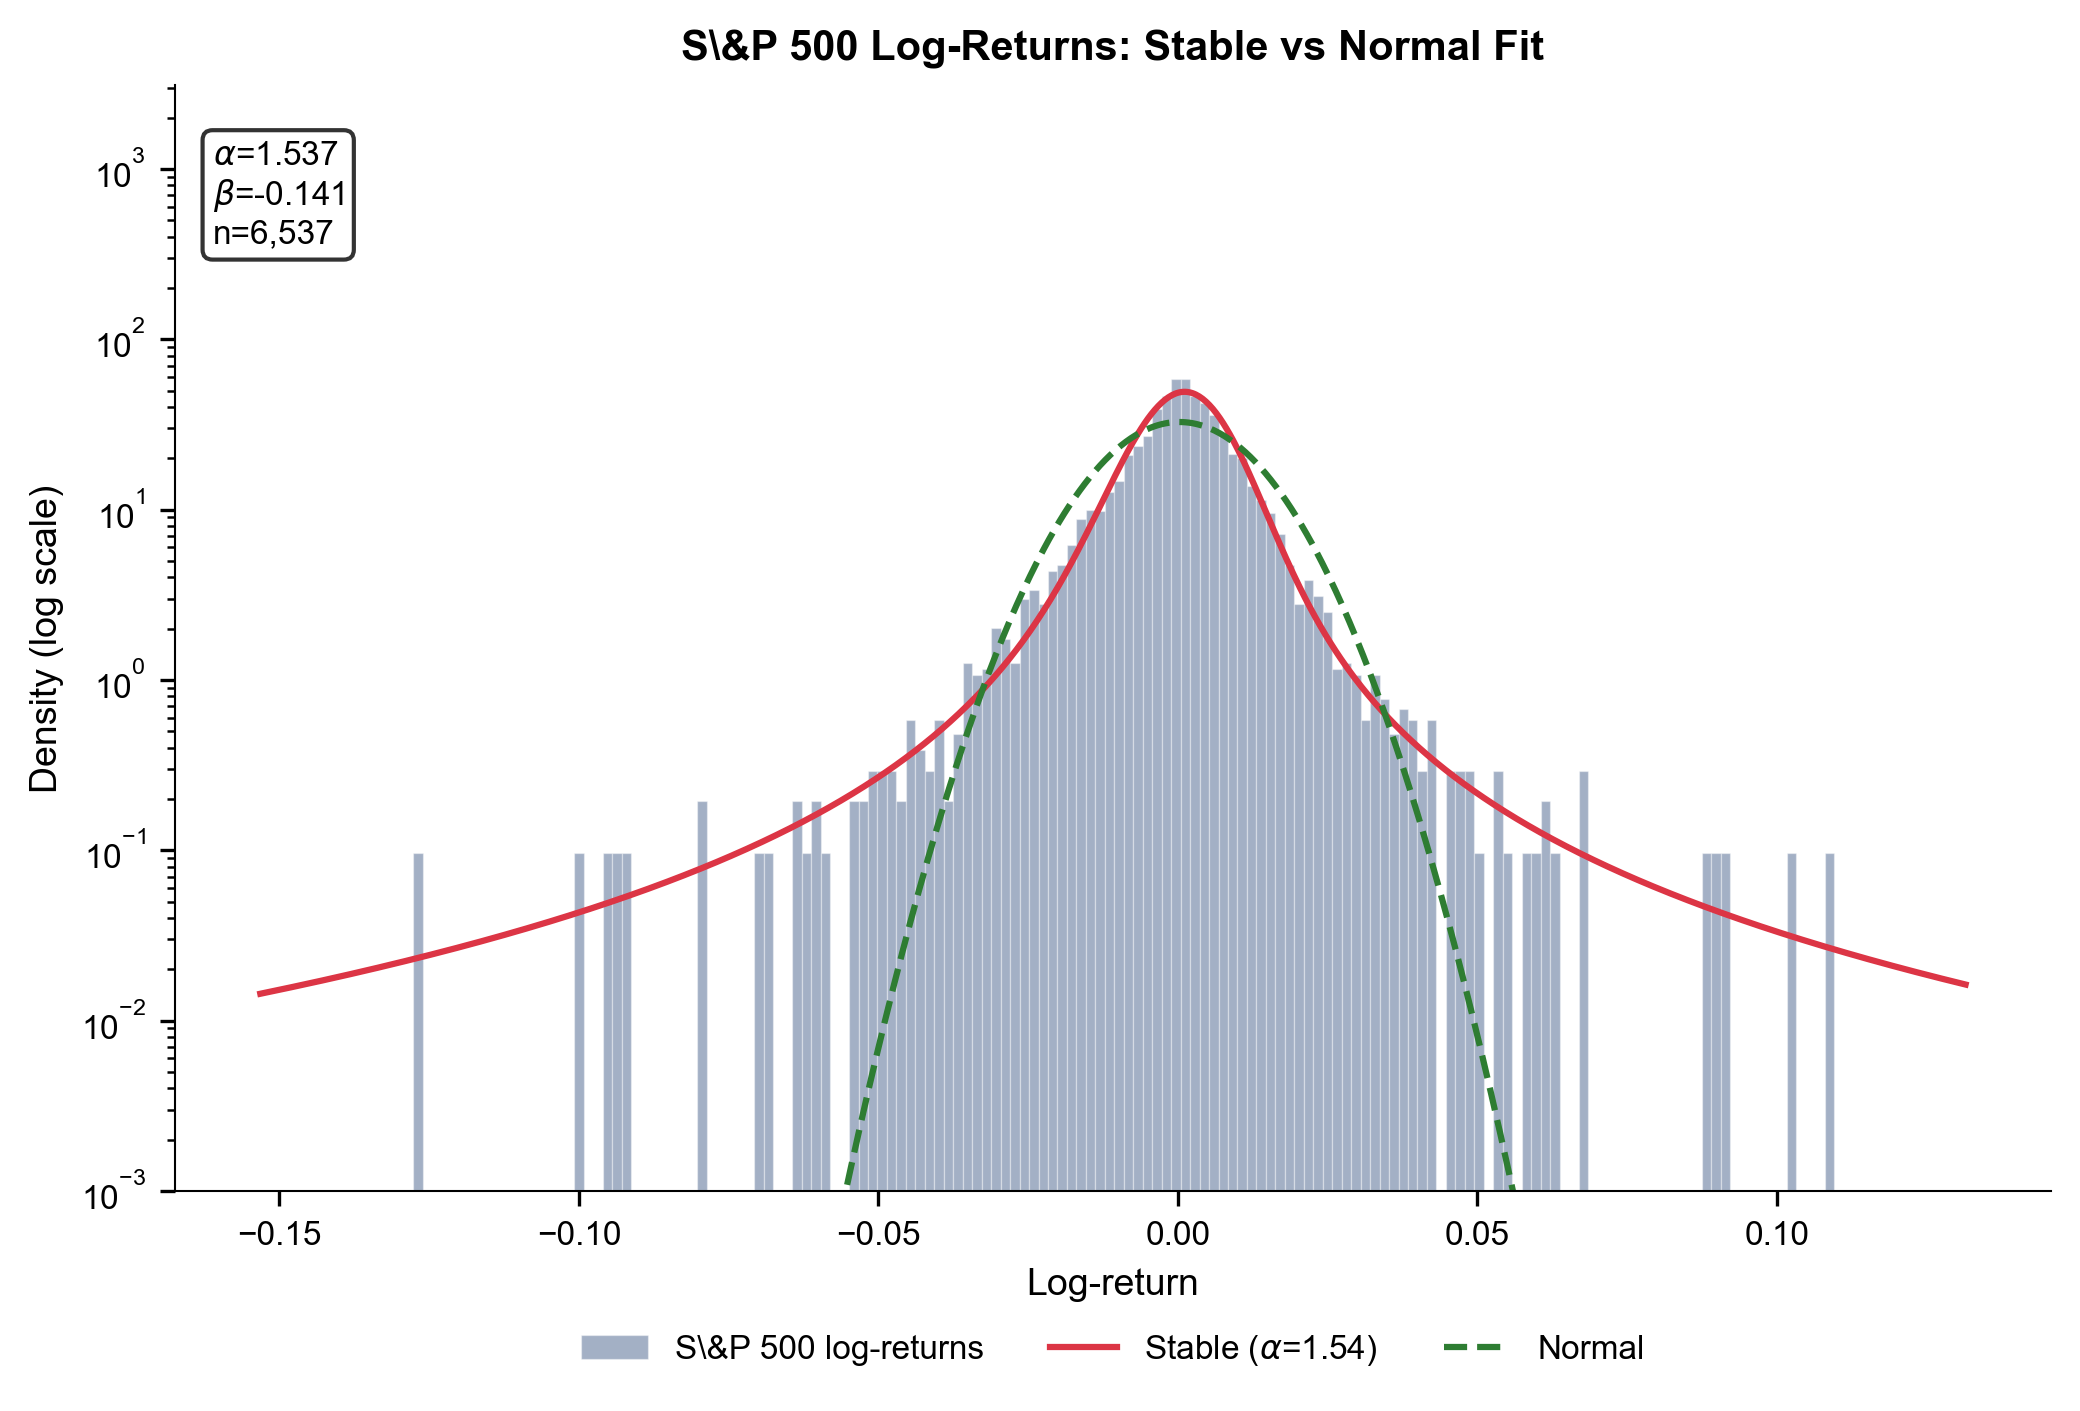
\includegraphics[width=0.78\textwidth]{ch2_sp500_stable_fit.png}
\end{center}

\vspace{-0.3cm}
\begin{itemize}\setlength{\itemsep}{0pt}
    \item Pe scară logaritmică, diferența în cozi este evidentă
    \item Distribuția stabilă captează \textbf{leptokurtosis} observată în date
    \item Distribuția normală subestimează probabilitățile din cozile distribuției
\end{itemize}
    \end{cminipage}
\end{frame}

\begin{frame}[fragile]{Python: VaR Comparison}

\begin{columns}[T]
\begin{column}{0.45\textwidth}
\begin{lstlisting}
# VaR comparison
levels = [0.01, 0.05, 0.001]
for cl in levels:
    var_s = levy_stable.ppf(
        cl, alpha, beta, loc, scale)
    var_n = norm.ppf(cl, mu, sigma)
    var_e = np.percentile(
        returns, cl*100)
    print(f"VaR {cl*100:.1f}%:")
    print(f"  Stable:    {var_s:.5f}")
    print(f"  Normal:    {var_n:.5f}")
    print(f"  Empirical: {var_e:.5f}")
\end{lstlisting}
\end{column}
\begin{column}{0.52\textwidth}
\begin{center}
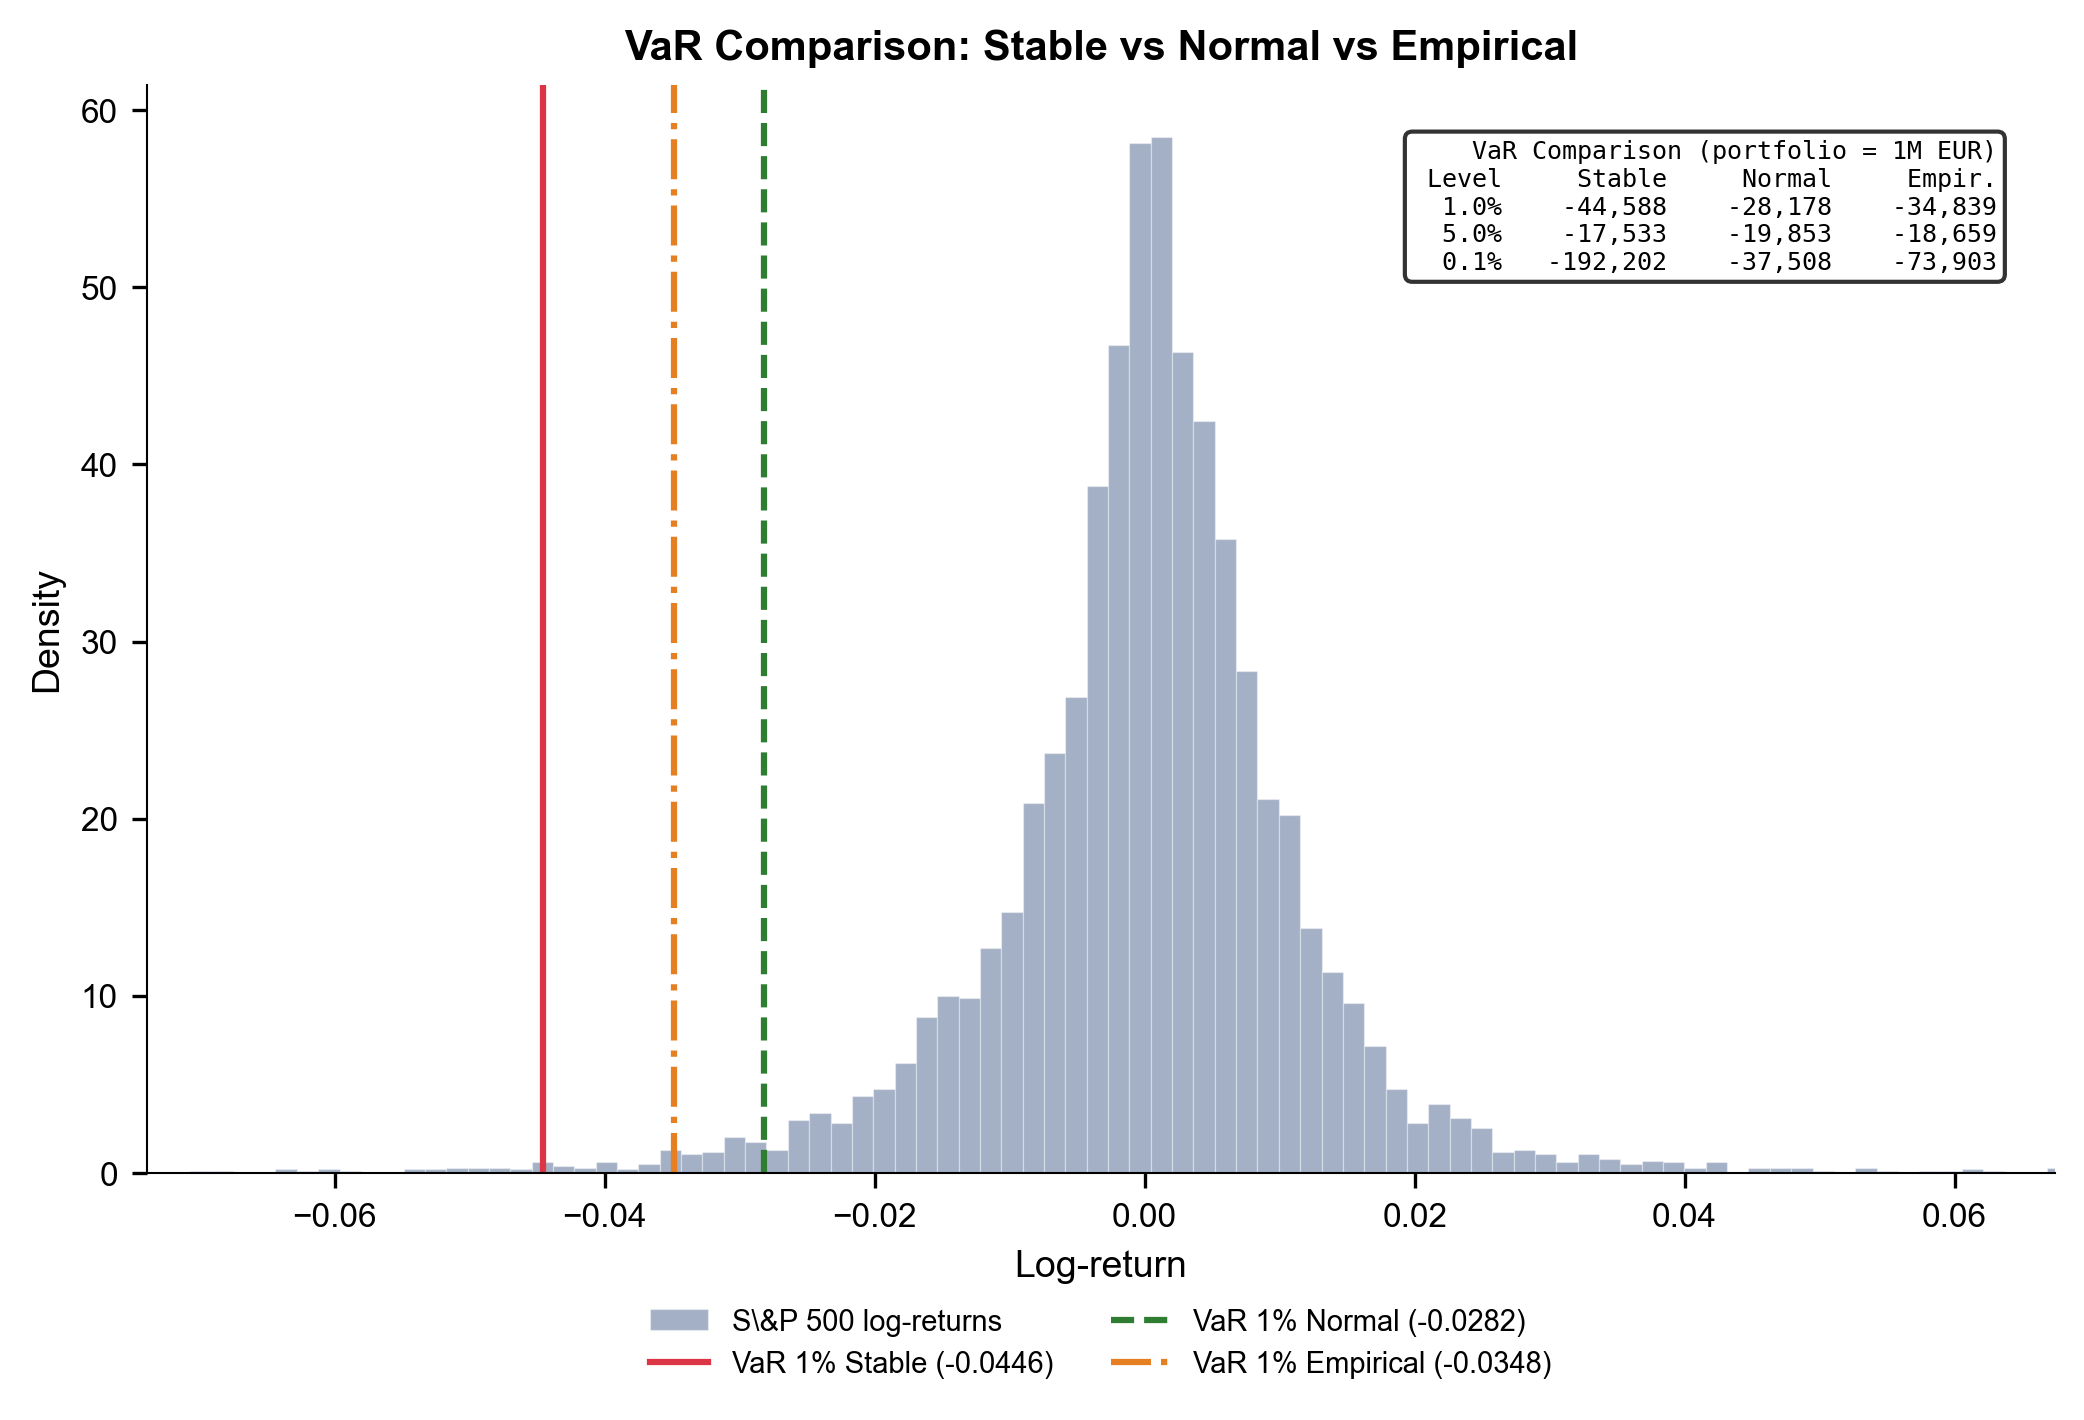
\includegraphics[width=\textwidth]{ch2_var_comparison.png}
\end{center}
\end{column}
\end{columns}
\end{frame}

\begin{frame}[fragile]{Exercițiu Python 5: Comparație Cross-Asset $\alpha$}
    \textbf{Sarcină:}
    \begin{enumerate}\setlength{\itemsep}{0pt}
        \item Descărcați randamente zilnice pentru S\&P 500, Bitcoin și Gold (ultimii 5 ani)
        \item Ajustați o distribuție stabilă pe fiecare activ
        \item Comparați $\hat{\alpha}$ --- care activ are cele mai grele cozi?
        \item Vizualizați PDF-urile estimate pe același grafic (log-scale)
    \end{enumerate}

    \vspace{0.3cm}
    \textbf{Cod cheie:}
    \begin{verbatim}
tickers = ['^GSPC', 'BTC-USD', 'GC=F']
for t in tickers:
    data = yf.download(t, start='2020-01-01')
    ret = np.log(data['Close']/data['Close'].shift(1)).dropna()
    a, b, loc, sc = levy_stable.fit(ret.values)
    print(f"{t}: alpha={a:.3f}, beta={b:.3f}")
    \end{verbatim}

    \quantlet{SFM\_ch2\_stable\_fit}{https://github.com/QuantLet/Stat_fin_markets/tree/master/Ch_02/SFM_ch2_stable_distributions}
\end{frame}

\begin{frame}[fragile]{Exercițiu Python 6: Backtesting VaR Stabil vs Normal}
    \textbf{Sarcină:}
    \begin{enumerate}\setlength{\itemsep}{0pt}
        \item Estimați VaR la 1\% pe o fereastră de 500 zile (rolling window)
        \item Comparați numărul de depășiri VaR: Normal vs Stabil vs Empiric
        \item Vizualizați randamentele cu liniile VaR suprapuse
    \end{enumerate}

    \vspace{0.3cm}
    \textbf{Cod cheie:}
    \begin{verbatim}
window = 500
for i in range(window, len(returns)):
    train = returns[i-window:i]
    a, b, loc, sc = levy_stable.fit(train)
    var_stable[i] = levy_stable.ppf(0.01, a, b, loc, sc)
    var_normal[i] = norm.ppf(0.01, train.mean(), train.std())
violations_s = (returns[window:] < var_stable[window:]).sum()
    \end{verbatim}

    \quantlet{SFM\_ch2\_stable\_fit}{https://github.com/QuantLet/Stat_fin_markets/tree/master/Ch_02/SFM_ch2_stable_distributions}
\end{frame}

\begin{frame}{Exercițiu AI: Prompt Engineering}
    \begin{cminipage}{0.95\textwidth}
\begin{block}{Exercițiu}
\begin{itemize}\setlength{\itemsep}{0pt}
    \item Folosiți ChatGPT sau Claude pentru a genera cod Python care:
\end{itemize}
\end{block}

\begin{enumerate}\setlength{\itemsep}{0pt}
    \item Descarcă datele BTC-USD din ultimii 5 ani
    \item Ajustează o distribuție stabilă pe log-randamentele zilnice
    \item Compară grafic PDF stabilă vs normală (log-scale)
    \item Calculează VaR la 1\% și 5\%
    \item Realizează un backtest: câte zile au depășit VaR-ul estimat?
\end{enumerate}

\vspace{0.3cm}
\begin{alertblock}{Prompt sugerat}
\begin{itemize}\setlength{\itemsep}{0pt}
    \item \textit{``Write Python code using scipy.stats.levy\_stable to fit a stable distribution to BTC-USD daily log-returns from yfinance. Plot histogram with stable and normal overlay on log-scale. Calculate VaR at 1\% and 5\% for both distributions and backtest against actual returns.''}
\end{itemize}
\end{alertblock}
    \end{cminipage}
\end{frame}

\begin{frame}{Discuție 1: Normal vs Stabil în Practică}
\begin{cminipage}{0.95\textwidth}
    \begin{itemize}\setlength{\itemsep}{0pt}
        \item \textbf{Scenariu:} Un fond de investiții folosește distribuția normală pentru calculul VaR zilnic. Auditorii recomandă trecerea la distribuția stabilă.
        \item \textbf{Întrebări:}
    \end{itemize}
    \begin{enumerate}\setlength{\itemsep}{0pt}
        \item Care sunt \textbf{avantajele} practice ale modelului normal? (simplitate, CLT, formulă închisă)
        \item Ce probleme specifice apar cu distribuția stabilă? (varianță infinită, estimare lentă, PDF fără formă închisă)
        \item La ce \textbf{nivel} de VaR (5\%, 1\%, 0.1\%) diferența contează cel mai mult?
        \item Cum justificați costul computațional suplimentar al modelului stabil?
    \end{enumerate}

    \vspace{0.2cm}
    \begin{block}{Recomandare}
        {\small Raportați ambele modele. Diferența este un \textbf{indicator} al riscului de model.}
    \end{block}
\end{cminipage}
\end{frame}

\begin{frame}{Discuție 2: Limitările Distribuțiilor Stabile}
\begin{cminipage}{0.95\textwidth}
    \begin{itemize}\setlength{\itemsep}{0pt}
        \item \textbf{Scenariu:} Estimați $\alpha = 1.6$ pe randamente zilnice BTC-USD. Managerul de risc întreabă: ``Sharpe ratio-ul portofoliului este 1.2. Este fiabil?''
        \item \textbf{Întrebări:}
    \end{itemize}
    \begin{enumerate}\setlength{\itemsep}{0pt}
        \item Cu $\alpha = 1.6$, ce momente \textbf{nu} există? Cum afectează aceasta Sharpe ratio-ul?
        \item Dacă varianța este infinită, cum comparați riscul între active?
        \item Ce \textbf{alternative} la Sharpe ratio funcționează cu distribuții stabile? (Rachev ratio, Stable Tail Adjusted Return)
        \item Distribuția stabilă presupune independență. Este realist pe piețele financiare?
    \end{enumerate}

    \vspace{0.2cm}
    \begin{itemize}\setlength{\itemsep}{0pt}
        \item \textbf{Indiciu:} Cu $\alpha = 1.6$, $\E[X^p] < \infty$ doar pentru $p < 1.6$. Varianța ($p=2$) este infinită.
    \end{itemize}
\end{cminipage}
\end{frame}

\begin{frame}{Exercițiu AI 2: Verificarea codului generat}
\begin{cminipage}{0.95\textwidth}
    \vspace{-3mm}
    \begin{block}{\footnotesize Prompt de testat}
        {\footnotesize
        ``Scrie cod Python care: (1) generează 10000 observații dintr-o distribuție stabilă cu alpha=1.5, beta=0.3, (2) estimează parametrii din eșantion folosind McCulloch și MLE, (3) compară estimările cu valorile reale, (4) vizualizează histograma cu PDF-ul estimat overlay.''
        }
    \end{block}
    \vspace{-2mm}
    {\footnotesize
    \begin{itemize}\setlength{\itemsep}{0pt}
        \item \textbf{Verificați:}
    \end{itemize}
    \begin{enumerate}\setlength{\itemsep}{0pt}
        \item LLM-ul folosește \texttt{levy\_stable.rvs()} corect (4 parametri: $\alpha, \beta, \text{loc}, \text{scale}$)?
        \item Implementarea McCulloch este corectă? (cuantile, nu momente!)
        \item MLE cu \texttt{levy\_stable.fit()} --- convergează? Rezultatele sunt rezonabile?
        \item Estimările sunt aproape de $\alpha = 1.5$, $\beta = 0.3$?
        \item Overlay-ul PDF folosește parametrii \textbf{estimați}, nu cei reali?
    \end{enumerate}
    }
    \vspace{-2mm}
    \begin{alertblock}{}
        {\footnotesize \textbf{Atenție}: \texttt{levy\_stable.fit()} poate fi foarte lent. Verificați dacă LLM-ul menționează această limitare.}
    \end{alertblock}
\end{cminipage}
\end{frame}

%=============================================================================
% STUDIU DE CAZ: S&P 500
%=============================================================================
\section{Studiu de caz: S\&P 500}

\begin{frame}{Histogram + Fit stabil vs Normal}
    \begin{cminipage}{0.95\textwidth}
\quantlet{SFM\_ch2\_stable\_fit}{https://github.com/QuantLet/Stat_fin_markets/tree/master/Ch_02/SFM_ch2_stable_distributions}

\begin{center}
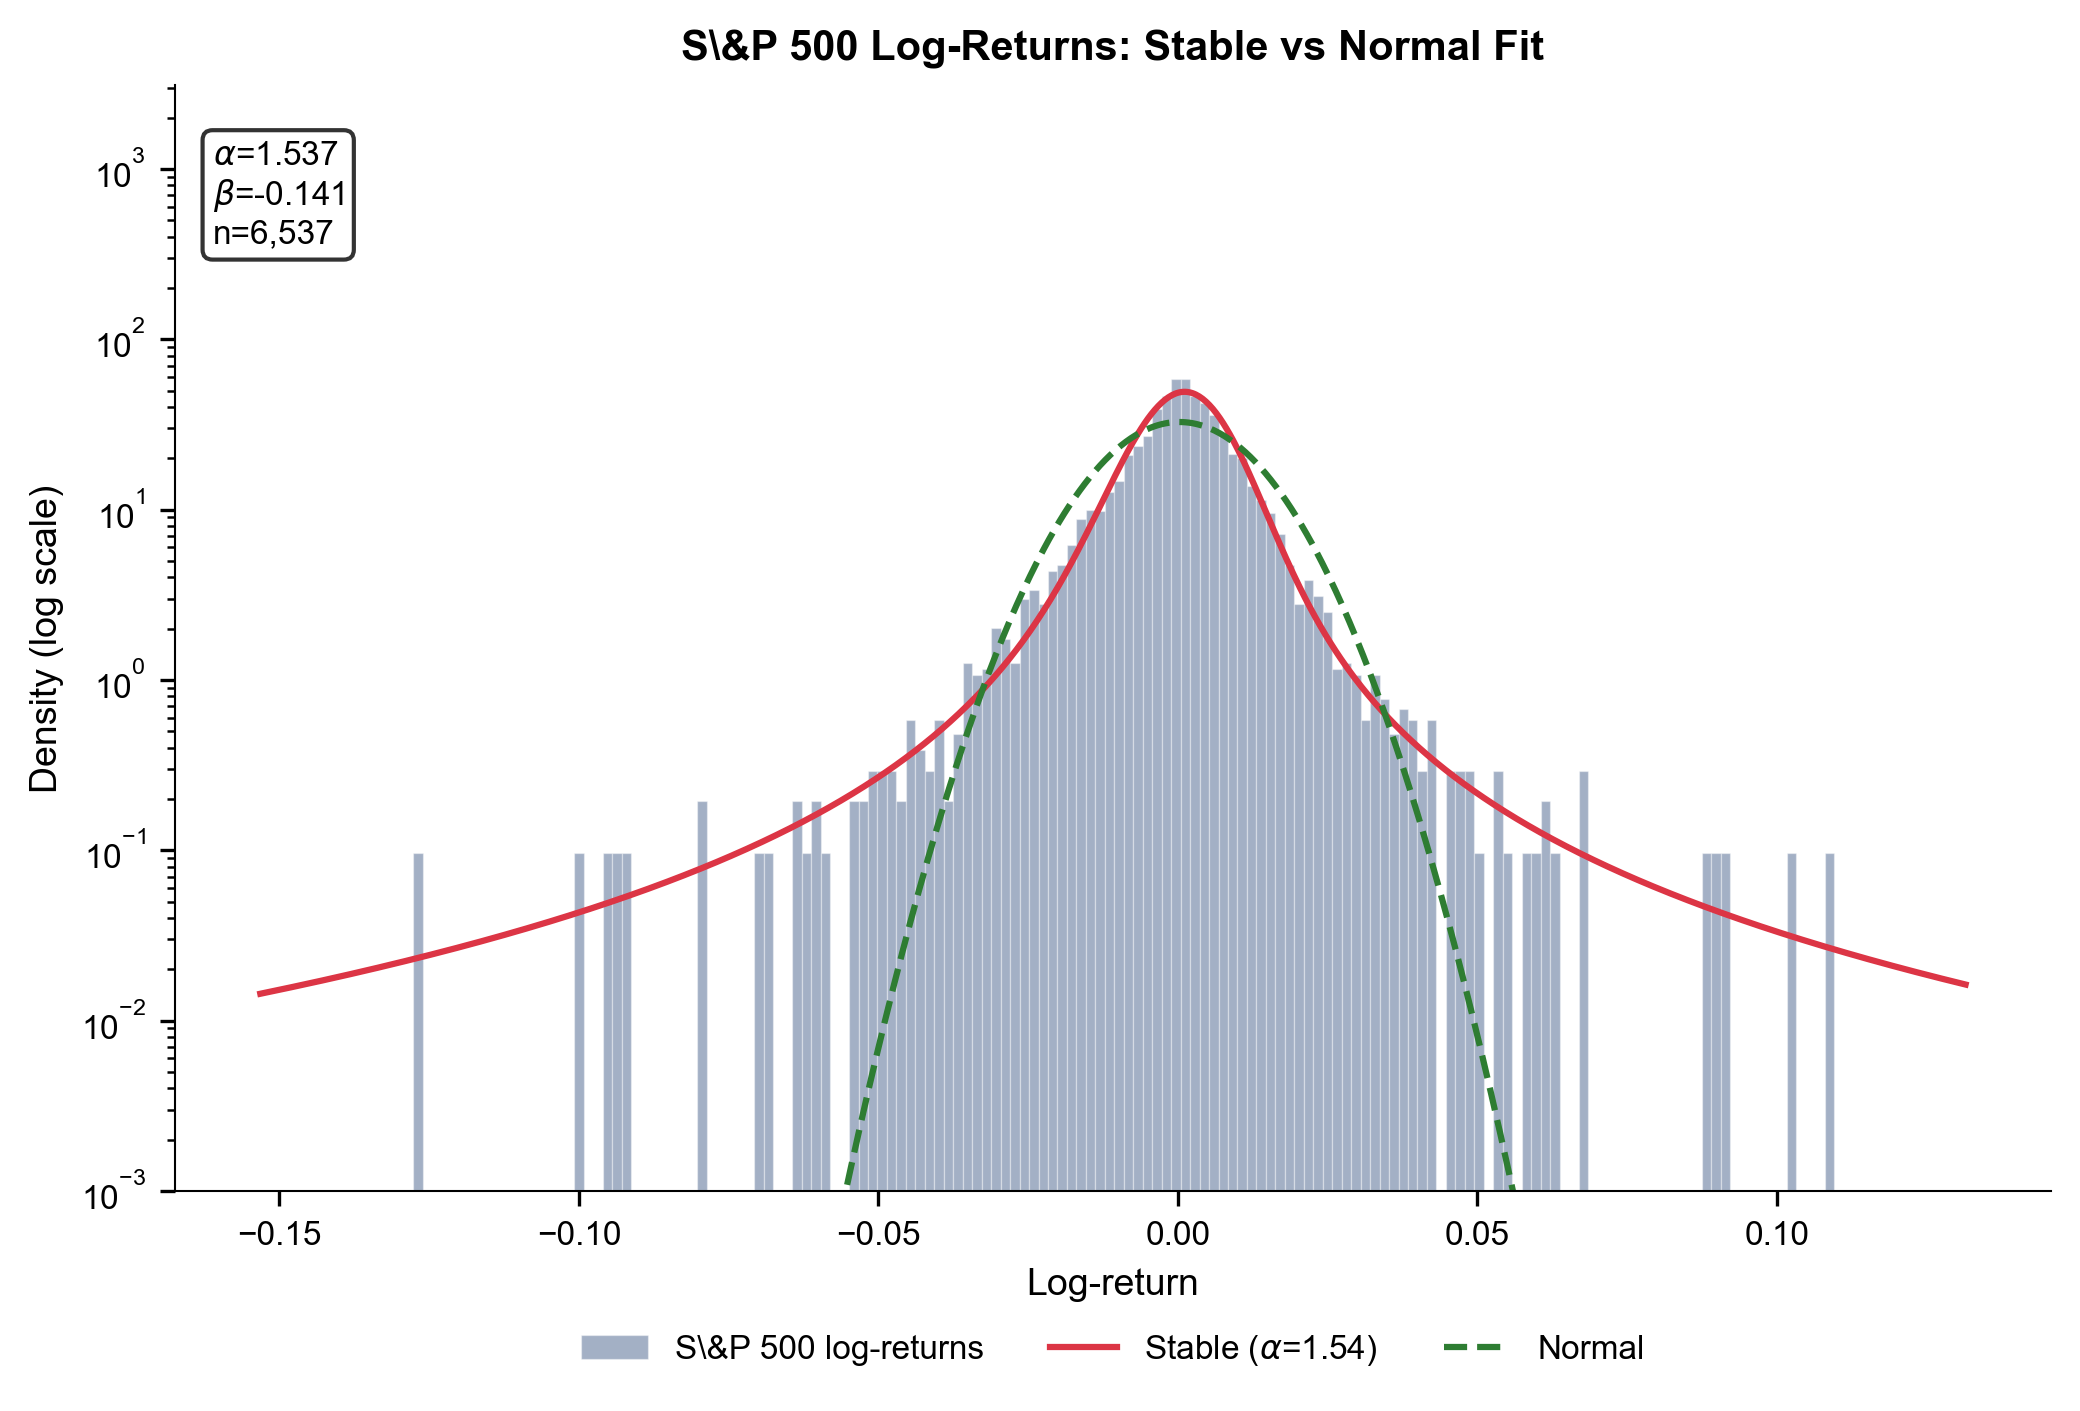
\includegraphics[width=0.85\textwidth]{ch2_sp500_stable_fit.png}
\end{center}

\vspace{-0.2cm}
\begin{itemize}\setlength{\itemsep}{0pt}
    \item Distribuția stabilă se potrivește mai bine în \textbf{centru} și în \textbf{cozi}
    \item Distribuția normală supraestimează densitatea la $\pm 1\sigma$ și subestimează în cozi
\end{itemize}
    \end{cminipage}
\end{frame}

\begin{frame}{Comparație PDF pe scară logaritmică}
    \begin{cminipage}{0.95\textwidth}
\quantlet{SFM\_ch2\_stable\_fit}{https://github.com/QuantLet/Stat_fin_markets/tree/master/Ch_02/SFM_ch2_stable_distributions}

\begin{columns}[T]
\begin{column}{0.55\textwidth}
\begin{center}
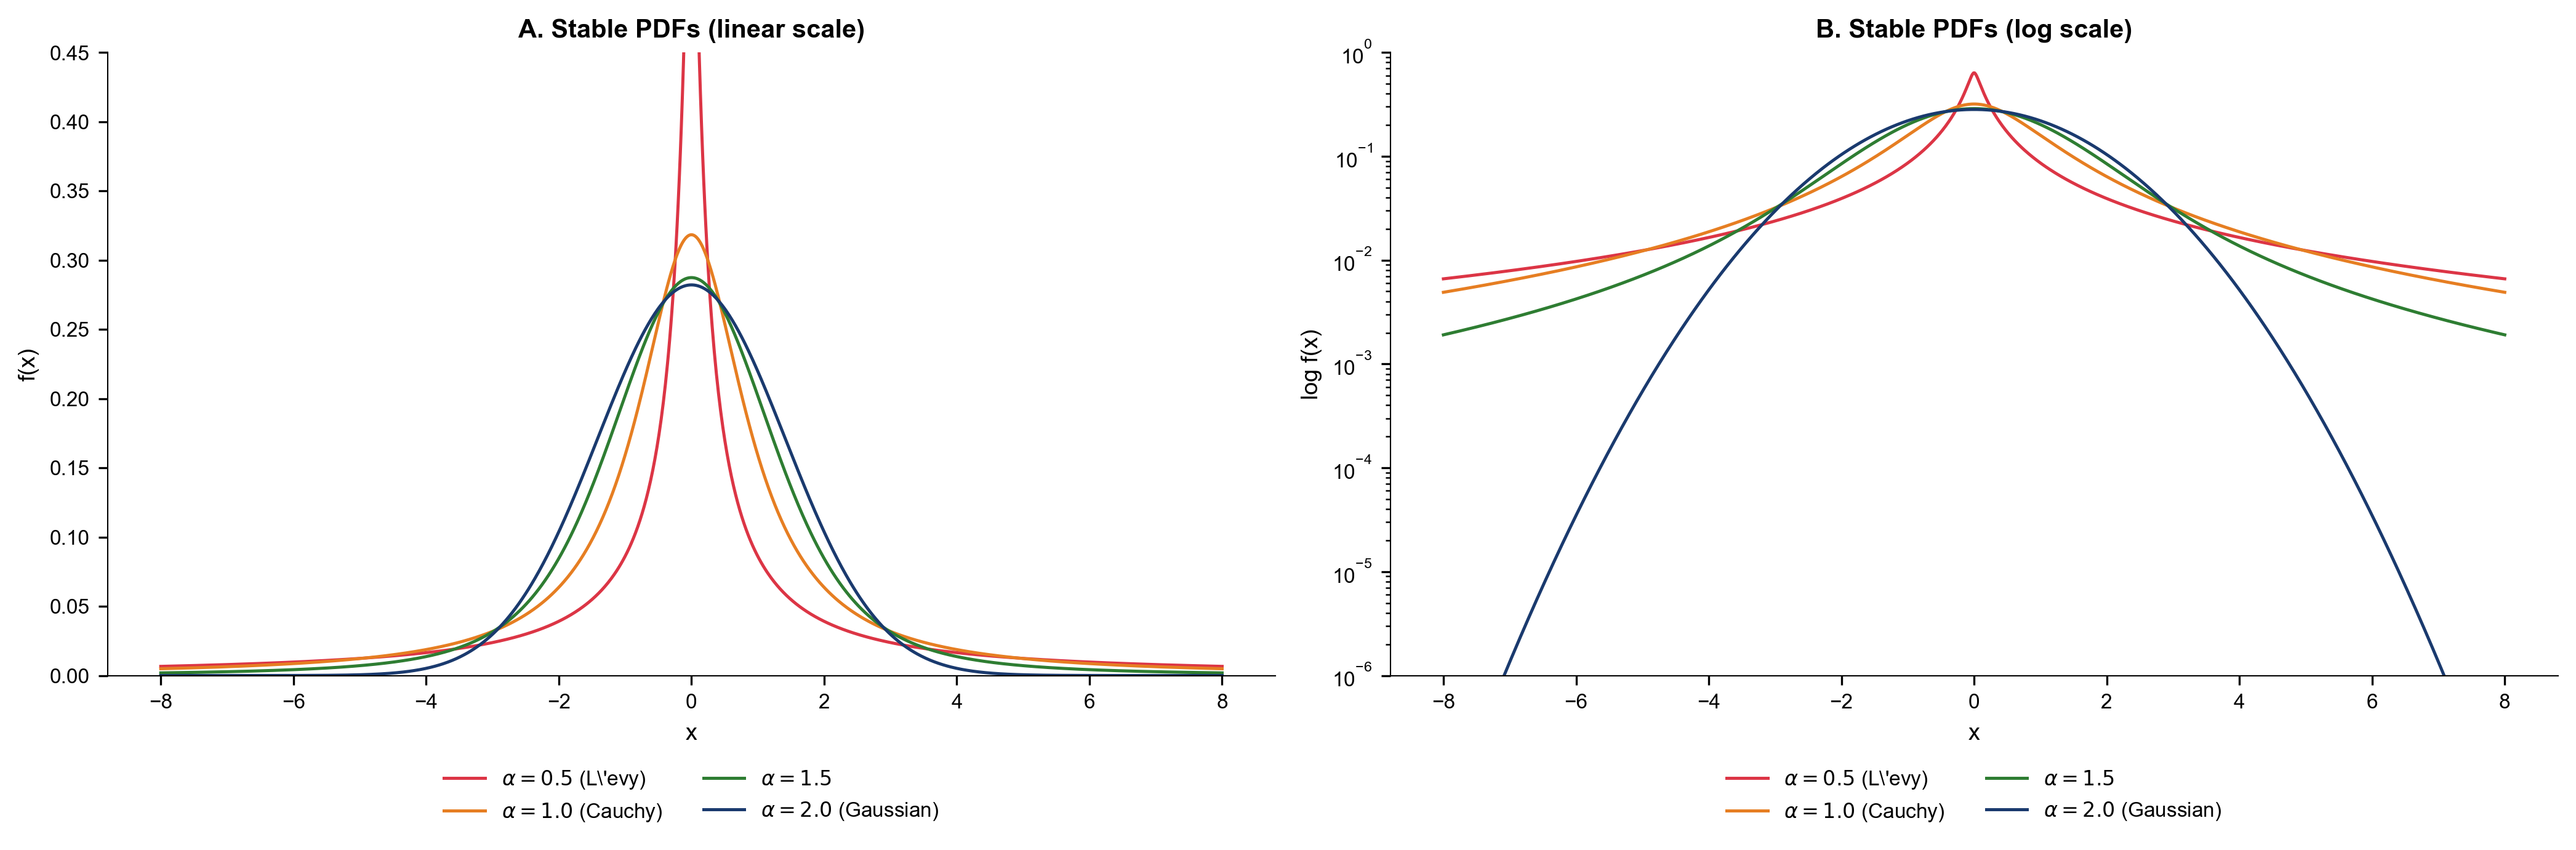
\includegraphics[width=\textwidth]{ch2_stable_pdfs.png}
\end{center}
\end{column}
\begin{column}{0.42\textwidth}
\begin{itemize}\setlength{\itemsep}{0pt}
    \item \textbf{Observații:}
    \item Panoul B (scară log) evidențiază diferențele din cozi
    \item Distribuția cu $\alpha = 0.5$ (L\'{e}vy) are cele mai grele cozi
    \item La $\alpha = 2.0$ se obține exact distribuția normală
    \item Randamentele financiare au de regulă $\alpha \in [1.5, 1.9]$
\end{itemize}
\end{column}
\end{columns}
    \end{cminipage}
\end{frame}

\begin{frame}{VaR: Tabel comparativ}
    \begin{cminipage}{0.95\textwidth}
\begin{block}{VaR pe S\&P 500 (2000--2025): Gaussiană vs Stabilă vs Empiric}
\renewcommand{\arraystretch}{1.3}
\begin{center}
\begin{tabular}{lccc}
\toprule
\textbf{Nivel VaR} & \textbf{Gaussiană} & \textbf{Stabilă} & \textbf{Empiric} \\
\midrule
5\% & $-1.91\%$ & $-2.14\%$ & $-2.08\%$ \\
1\% & $-2.71\%$ & $-4.12\%$ & $-3.56\%$ \\
0.1\% & $-3.59\%$ & $-8.97\%$ & $-6.88\%$ \\
\bottomrule
\end{tabular}
\end{center}
\end{block}

\begin{itemize}\setlength{\itemsep}{0pt}
    \item La nivelul de 5\%, diferențele sunt mici
    \item La 1\%, modelul stabil este cu $\sim$50\% mai conservator decât Gaussiana
    \item La 0.1\%, modelul stabil estimează pierderi de \textbf{2.5$\times$} mai mari
    \item VaR-ul empiric se situează \textbf{între} cele două modele parametrice
\end{itemize}
    \end{cminipage}
\end{frame}

\begin{frame}{Comparație cross-asset: Indicele de stabilitate $\alpha$}
    \begin{cminipage}{0.95\textwidth}
\quantlet{SFM\_ch2\_stable\_fit}{https://github.com/QuantLet/Stat_fin_markets/tree/master/Ch_02/SFM_ch2_stable_distributions}

\begin{center}
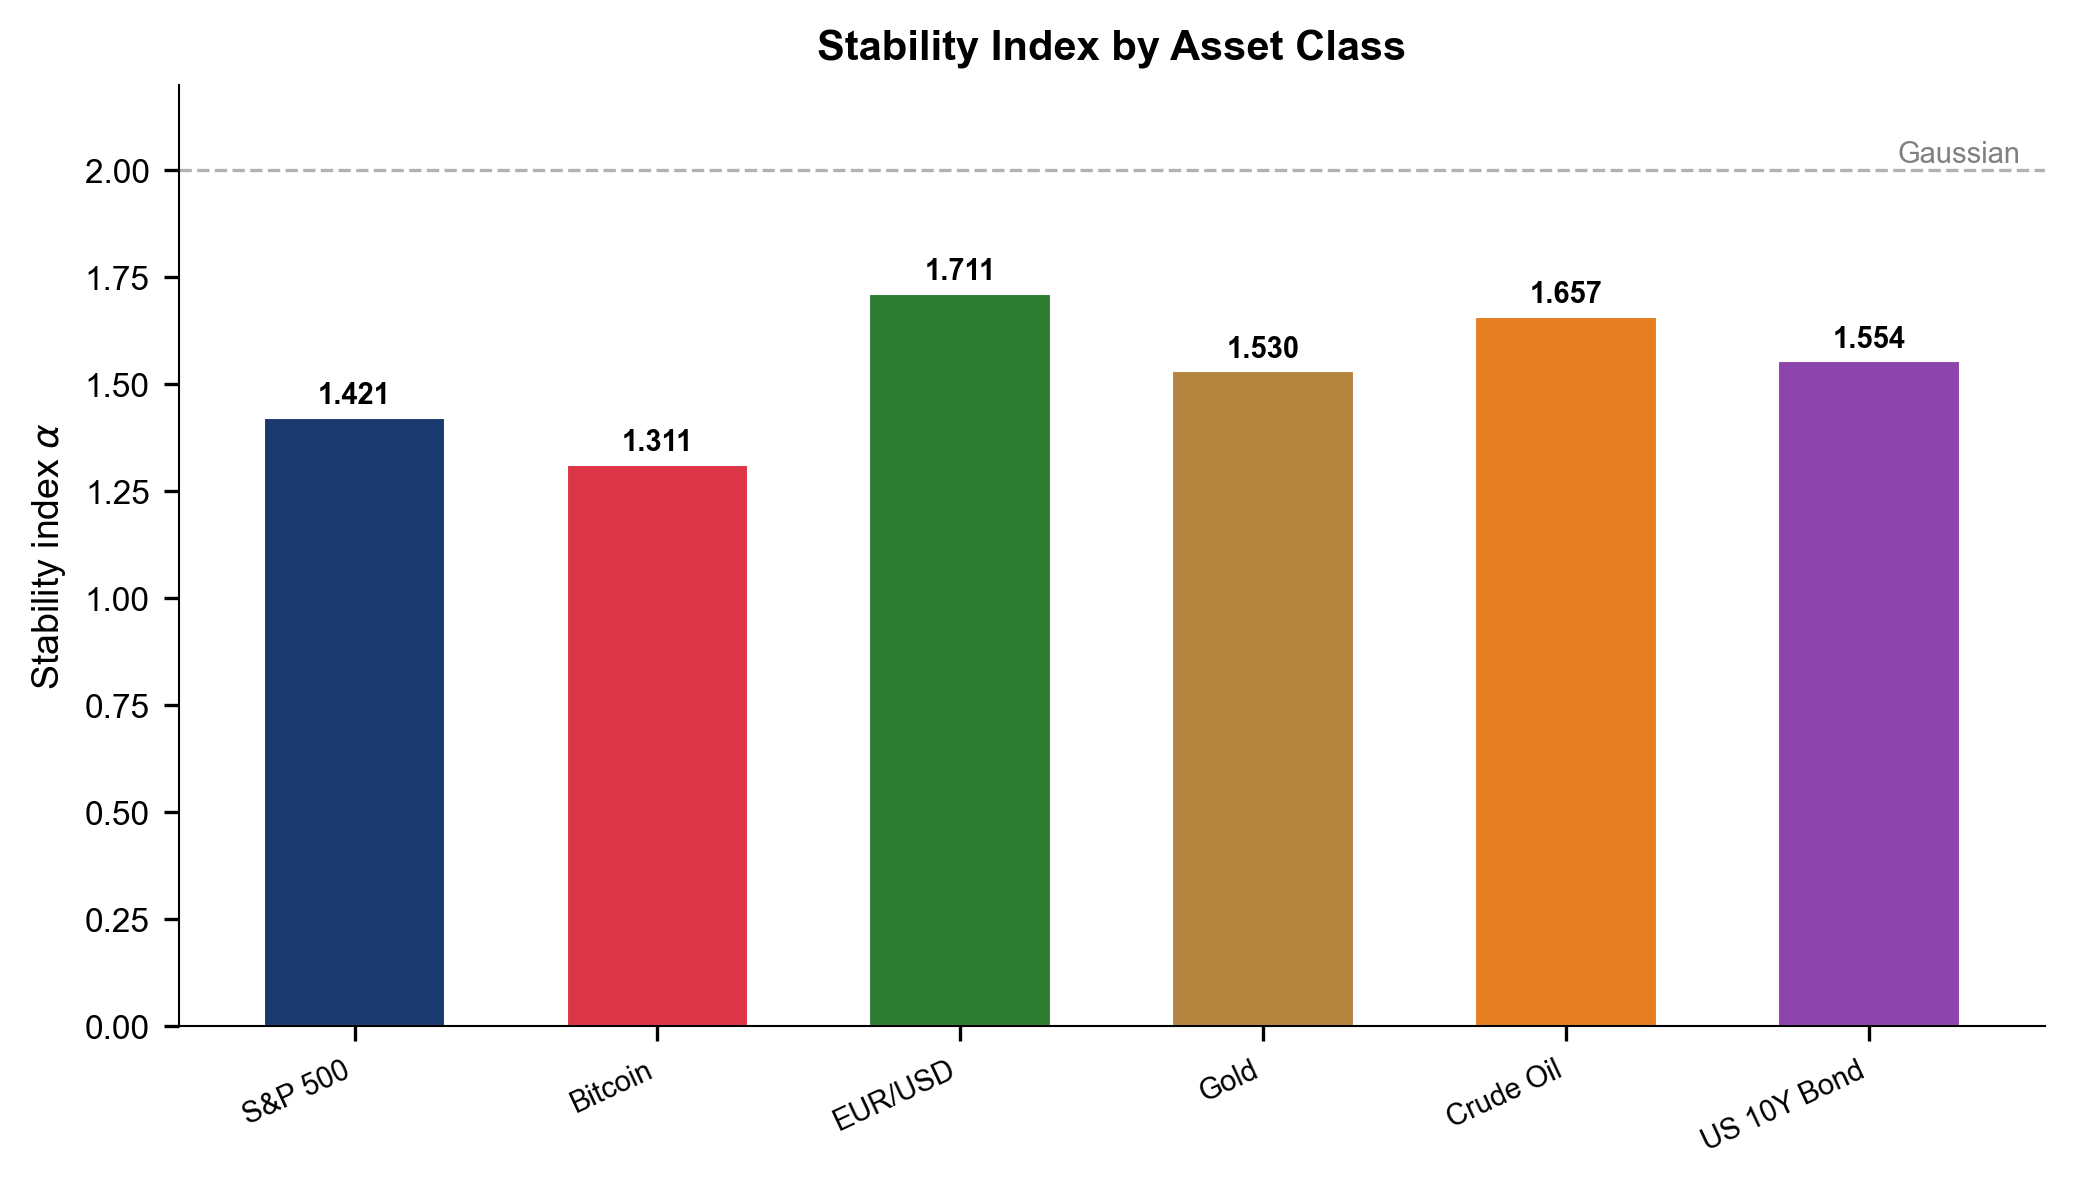
\includegraphics[width=0.75\textwidth]{ch2_cross_asset_alpha.png}
\end{center}

\vspace{-0.2cm}
\begin{itemize}\setlength{\itemsep}{0pt}
    \item Bitcoin are cel mai mic $\alpha$ $\Rightarrow$ cele mai grele cozi
    \item Obligațiunile au $\alpha$ cel mai mare (aproape Gaussian)
    \item \textbf{Nicio} clasă de active nu este perfect Gaussiană ($\alpha < 2$)
\end{itemize}
    \end{cminipage}
\end{frame}

%=============================================================================
% TEMĂ
%=============================================================================
\section{Tema pentru acasă}

\begin{frame}{Temă: Distribuții stabile pe BVB}
    \begin{cminipage}{0.95\textwidth}
\begin{block}{Cerințe}
\begin{enumerate}\setlength{\itemsep}{0pt}
    \item Alegeți o acțiune listată la BVB (ex: TLV, SNP, BRD, FP)
    \item Descărcați datele zilnice din ultimii 5 ani
    \item Ajustați o distribuție stabilă pe log-randamente
    \item Comparați grafic PDF stabilă vs normală (scară logaritmică)
    \item Calculați VaR la 1\% și 5\% (stabil vs normal vs empiric)
    \item Interpretați rezultatele: este piața românească ``mai Gaussiană'' decât S\&P 500?
\end{enumerate}
\end{block}

\vspace{0.2cm}
\begin{exampleblock}{Indicii}
\begin{itemize}\setlength{\itemsep}{0pt}
    \item Folosiți \texttt{yfinance} cu ticker-ul BVB (ex: \texttt{TLV.RO})
    \item Funcția \texttt{levy\_stable.fit()} poate fi lentă --- folosiți \texttt{floc=np.mean(data)}
    \item Comparați $\alpha$ estimat cu cel al S\&P 500
\end{itemize}
\end{exampleblock}
    \end{cminipage}
\end{frame}

%=============================================================================
% REZUMAT
%=============================================================================
\section{Rezumat}

\begin{frame}{Checklist competențe}
    \begin{cminipage}{0.95\textwidth}
\begin{columns}[T]
\begin{column}{0.48\textwidth}
\begin{block}{Teorie}
\begin{itemize}\setlength{\itemsep}{0pt}
    \item[$\square$] Definiția stabilității prin sume
    \item[$\square$] Parametrii: $\alpha$, $\beta$, $\gamma$, $\delta$
    \item[$\square$] Cazuri speciale: Gauss, Cauchy, L\'{e}vy
    \item[$\square$] Funcția caracteristică
    \item[$\square$] Existența momentelor ($p < \alpha$)
    \item[$\square$] Comportamentul cozilor (lege putere)
\end{itemize}
\end{block}
\end{column}
\begin{column}{0.48\textwidth}
\begin{block}{Practică}
\begin{itemize}\setlength{\itemsep}{0pt}
    \item[$\square$] Estimarea McCulloch (cuantile)
    \item[$\square$] MLE cu \texttt{levy\_stable.fit()}
    \item[$\square$] Regresia Koutrouvelis (ECF)
    \item[$\square$] VaR: stabil vs normal vs empiric
    \item[$\square$] Simulare și vizualizare în Python
    \item[$\square$] Interpretarea $\alpha$ pe date reale
\end{itemize}
\end{block}
\end{column}
\end{columns}

    \vspace{0.3cm}
    \begin{block}{Următorul Seminar}
        Cozi Grele --- Skew-$t$, GED și EVT
    \end{block}
    \end{cminipage}
\end{frame}

%=============================================================================
% PLANIFICAREA SEMINARELOR
%=============================================================================
\section{Planificarea seminarelor}

\begin{frame}{Planificarea seminarelor}
    \begin{cminipage}{0.95\textwidth}
\renewcommand{\arraystretch}{1.3}
\begin{center}
\begin{tabular}{clll}
\toprule
\textbf{Săpt.} & \textbf{Tema} & \textbf{Curs asociat} & \textbf{Conținut principal} \\
\midrule
1 & Randamente & Cap. 1: Surse de date & Tipuri randamente, staționaritate \\
2 & Distribuții clasice & Cap. 2: Distribuții & Normal, Student-$t$, Pareto, VaR \\
\rowcolor{MainBlue!10}
\textbf{3} & \textbf{Distribuții stabile} & \textbf{Cap. 2: Distribuții} & \textbf{Fit stabil, VaR, cozi grele} \\
4 & Cozi grele & Cap. 2: Distribuții & Skew-$t$, GED, EVT \\
5 & Selecția modelului & Cap. 2: Distribuții & AIC/BIC, backtesting VaR \\
\bottomrule
\end{tabular}
\end{center}
    \end{cminipage}
\end{frame}

%=============================================================================
% TEST RAPID
%=============================================================================
\section{Test rapid}

\begin{frame}{Quiz: 5 întrebări}
    \begin{cminipage}{0.95\textwidth}
\begin{enumerate}\setlength{\itemsep}{0pt}
    \item Care sunt limitele parametrului de stabilitate $\alpha$?
    \begin{enumerate}\setlength{\itemsep}{0pt}
        \item[(a)] $0 < \alpha \leq 1$
        \item[(b)] $0 < \alpha \leq 2$
        \item[(c)] $-2 \leq \alpha \leq 2$
        \item[(d)] $\alpha > 0$
    \end{enumerate}

    \vspace{0.2cm}
    \item Pentru o distribuție $S(1.6, 0, 1, 0)$, care momente \textbf{există}?
    \begin{enumerate}\setlength{\itemsep}{0pt}
        \item[(a)] Media și varianța
        \item[(b)] Doar media
        \item[(c)] Toate momentele
        \item[(d)] Niciun moment
    \end{enumerate}

    \vspace{0.2cm}
    \item Ce distribuție se obține la $\alpha = 1, \beta = 0$?
    \begin{enumerate}\setlength{\itemsep}{0pt}
        \item[(a)] Gaussiană
        \item[(b)] Cauchy
        \item[(c)] L\'{e}vy
        \item[(d)] Exponențială
    \end{enumerate}
\end{enumerate}
    \end{cminipage}
\end{frame}

\begin{frame}{Quiz: 5 întrebări (cont.) + Răspunsuri}
    \begin{cminipage}{0.95\textwidth}
\begin{enumerate}\setlength{\itemsep}{0pt}
    \setcounter{enumi}{3}
    \item În metoda McCulloch, $v_\alpha = 2.44$ corespunde:
    \begin{enumerate}\setlength{\itemsep}{0pt}
        \item[(a)] Cauchy
        \item[(b)] Gaussiană
        \item[(c)] L\'{e}vy
        \item[(d)] Stabil($\alpha = 1.5$)
    \end{enumerate}

    \vspace{0.2cm}
    \item De ce VaR stabil $>$ VaR Gaussian la 0.1\%?
    \begin{enumerate}\setlength{\itemsep}{0pt}
        \item[(a)] Distribuția stabilă are cozi mai grele
        \item[(b)] Distribuția stabilă este mai simetrică
        \item[(c)] Gaussiana are varianță infinită
        \item[(d)] Parametrul $\beta$ este negativ
    \end{enumerate}
\end{enumerate}

\vspace{0.3cm}
\begin{exampleblock}{Răspunsuri}
\begin{enumerate}\setlength{\itemsep}{0pt}
    \item \textbf{(b)} $0 < \alpha \leq 2$
    \item \textbf{(b)} Doar media (deoarece $p < \alpha = 1.6$, deci doar $p < 1.6$)
    \item \textbf{(b)} Cauchy
    \item \textbf{(b)} Gaussiană ($\alpha = 2.0$)
    \item \textbf{(a)} Cozile mai grele ale distribuției stabile
\end{enumerate}
\end{exampleblock}
    \end{cminipage}
\end{frame}

\begin{frame}{Test 6: Proprietatea de stabilitate}
\begin{cminipage}{0.95\textwidth}
    \begin{alertblock}{Întrebare}
        Dacă $X_1, X_2 \sim S(\alpha, \beta, \gamma, \delta)$ i.i.d., atunci $X_1 + X_2$ este:
    \end{alertblock}

    \vspace{0.5cm}
    \begin{block}{Variante de răspuns}
    \textcolor{MainBlue}{\textbf{(A)}} $S(\alpha, \beta, 2\gamma, 2\delta)$\\[3pt]
    \textcolor{MainBlue}{\textbf{(B)}} $S(2\alpha, \beta, \gamma, \delta)$\\[3pt]
    \textcolor{MainBlue}{\textbf{(C)}} $S(\alpha, \beta, 2^{1/\alpha}\gamma, 2\delta)$\\[3pt]
    \textcolor{MainBlue}{\textbf{(D)}} $S(\alpha, 2\beta, \gamma, \delta)$
    \end{block}
\end{cminipage}
\end{frame}

\begin{frame}{Test 6: Răspuns}
\begin{cminipage}{0.95\textwidth}
    \begin{exampleblock}{Răspuns: C}
        $X_1 + X_2 \sim S(\alpha, \beta, 2^{1/\alpha}\gamma, 2\delta)$
    \end{exampleblock}

    \vspace{0.2cm}

    \begin{itemize}\setlength{\itemsep}{0pt}
        \item \textbf{Regula generală de stabilitate:}
        \item Dacă $X_1, \ldots, X_n$ sunt i.i.d.\ $S(\alpha, \beta, \gamma, \delta)$:
    \end{itemize}
    $$X_1 + \cdots + X_n \sim S(\alpha, \beta, n^{1/\alpha}\gamma, n\delta)$$
    \begin{itemize}\setlength{\itemsep}{0pt}
        \item $\alpha$ și $\beta$ se \textbf{păstrează} (forma și asimetria)
        \item $\gamma$ (scara) crește cu factorul $n^{1/\alpha}$
        \item $\delta$ (locația) se adună liniar
        \item \textbf{Verificare:} $\alpha = 2$ (Normal): $n^{1/2}\gamma = \sqrt{n}\,\sigma$ \correct
        \item $\alpha = 1$ (Cauchy): $n^{1/1}\gamma = n\gamma$ --- scara crește \textbf{liniar}!
    \end{itemize}
\end{cminipage}
\end{frame}

\begin{frame}{Test 7: Convergența la distribuție stabilă}
\begin{cminipage}{0.95\textwidth}
    \begin{alertblock}{Întrebare}
        Fie $X_1, \ldots, X_n$ i.i.d.\ cu $\alpha = 1.7$. Ce se întâmplă cu media $\bar{X}_n$ când $n \to \infty$?
    \end{alertblock}

    \vspace{0.5cm}
    \begin{block}{Variante de răspuns}
    \textcolor{MainBlue}{\textbf{(A)}} Converge la Normal (CLT clasic funcționează)\\[3pt]
    \textcolor{MainBlue}{\textbf{(B)}} Converge la distribuție stabilă cu același $\alpha$\\[3pt]
    \textcolor{MainBlue}{\textbf{(C)}} Converge la Cauchy\\[3pt]
    \textcolor{MainBlue}{\textbf{(D)}} Nu converge la nimic
    \end{block}
\end{cminipage}
\end{frame}

\begin{frame}{Test 7: Răspuns}
\begin{cminipage}{0.95\textwidth}
    \begin{exampleblock}{Răspuns: B}
        Media converge la o distribuție stabilă cu același $\alpha = 1.7$
    \end{exampleblock}

    \vspace{0.2cm}

    \begin{itemize}\setlength{\itemsep}{0pt}
        \item \textbf{CLT generalizat (Gnedenko--Kolmogorov):}
        \item Dacă $\Var(X) = \infty$ ($\alpha < 2$), CLT clasic \textbf{nu se aplică}
        \item Media normalizată converge la o distribuție \textbf{stabilă}:
    \end{itemize}
    $$\frac{X_1 + \cdots + X_n - n\delta}{n^{1/\alpha}\gamma} \xrightarrow{d} S(\alpha, \beta, 1, 0)$$
    \begin{itemize}\setlength{\itemsep}{0pt}
        \item Normalizarea este $n^{1/\alpha}$, nu $\sqrt{n}$
        \item $\alpha = 1.7$: viteza de convergență este $n^{1/1.7} \approx n^{0.59}$
        \item $\Rightarrow$ Distribuțiile stabile sunt singurele \textbf{atractori} posibili pentru sume normalizate
    \end{itemize}
\end{cminipage}
\end{frame}

\begin{frame}{Test 8: Estimatorul McCulloch}
\begin{cminipage}{0.95\textwidth}
    \begin{alertblock}{Întrebare}
        Statisticile McCulloch $v_\alpha$ și $v_\beta$ se calculează din:
    \end{alertblock}

    \vspace{0.5cm}
    \begin{block}{Variante de răspuns}
    \textcolor{MainBlue}{\textbf{(A)}} Momentele eșantionului (medie, varianță, skewness)\\[3pt]
    \textcolor{MainBlue}{\textbf{(B)}} Cuantilele eșantionului ($q_{0.05}$, $q_{0.25}$, $q_{0.50}$, $q_{0.75}$, $q_{0.95}$)\\[3pt]
    \textcolor{MainBlue}{\textbf{(C)}} Funcția caracteristică empirică\\[3pt]
    \textcolor{MainBlue}{\textbf{(D)}} Log-verosimilitatea maximă
    \end{block}
\end{cminipage}
\end{frame}

\begin{frame}{Test 8: Răspuns}
\begin{cminipage}{0.95\textwidth}
    \begin{exampleblock}{Răspuns: B}
        McCulloch folosește 5 cuantile ale eșantionului
    \end{exampleblock}

    \vspace{0.2cm}

    \begin{itemize}\setlength{\itemsep}{0pt}
        \item \textbf{De ce cuantile și nu momente?}
        \item Momentele de ordin $\geq \alpha$ sunt \textbf{infinite} $\Rightarrow$ inutilizabile
        \item Cuantilele există \textbf{întotdeauna}, indiferent de $\alpha$
        \item \textbf{Cele 5 cuantile:} $q_{0.05}$, $q_{0.25}$, $q_{0.50}$, $q_{0.75}$, $q_{0.95}$
    \end{itemize}
    $$v_\alpha = \frac{q_{0.95} - q_{0.05}}{q_{0.75} - q_{0.25}}, \qquad v_\beta = \frac{q_{0.95} + q_{0.05} - 2q_{0.50}}{q_{0.95} - q_{0.05}}$$
    \begin{itemize}\setlength{\itemsep}{0pt}
        \item A: Momentele nu funcționează (pot fi infinite) \incorrect
        \item C: Metoda Koutrouvelis, nu McCulloch \incorrect
        \item D: MLE, nu McCulloch \incorrect
    \end{itemize}
\end{cminipage}
\end{frame}

%=============================================================================
% BIBLIOGRAFIE
%=============================================================================
\section{Bibliografie}

\begin{frame}{Bibliografie I}
    \begin{cminipage}{0.95\textwidth}
    \begin{block}{Distribuții Stabile}
        {\small
        \begin{itemize}\setlength{\itemsep}{0pt}
            \item Nolan, J.P. (2020). \textit{Stable Distributions: Models for Heavy Tailed Data}, Birkh\"{a}user.
            \item Mandelbrot, B. (1963). ``The variation of certain speculative prices,'' \textit{Journal of Business}, 36(4).
            \item Rachev, S.T., Mittnik, S. (2000). \textit{Stable Paretian Models in Finance}, Wiley.
            \item Franke, J., H\"{a}rdle, W.K., Hafner, C.M. (2019). \textit{Statistics of Financial Markets}, 4th ed., Springer.
            \item McCulloch, J.H. (1986). ``Simple consistent estimators of stable distribution parameters,'' \textit{Communications in Statistics --- Simulation and Computation}, 15(4).
        \end{itemize}
        }
    \end{block}

    \begin{exampleblock}{Resurse online}
        {\small
        \begin{itemize}\setlength{\itemsep}{0pt}
            \item \url{https://quantlet.com} --- Quantlet repository
            \item \url{https://danpele.github.io/SFM/} --- Materialele cursului
        \end{itemize}
        }
    \end{exampleblock}
    \end{cminipage}
\end{frame}

%=============================================================================
% MULȚUMESC
%=============================================================================
\begin{frame}{}
    \begin{cminipage}{0.95\textwidth}
    \centering
    \Huge\textcolor{IDAred}{Vă mulțumesc!}
    \vspace{1cm}
    \Large\textcolor{MainBlue}{Întrebări?}
    \vspace{0.8cm}
    \normalsize
    Materialele seminarului sunt disponibile la: \url{https://danpele.github.io/SFM/}
    \vspace{0.2cm}
    \href{https://quantlet.com}{\raisebox{-0.15em}{
\includegraphics[height=0.8em]{ql_logo.png}} Quantlet} \hspace{0.5cm}
    \href{https://quantinar.com}{\raisebox{-0.15em}{
\includegraphics[height=0.8em]{qr_logo.png}} Quantinar}
    \end{cminipage}
\end{frame}

\end{document}
